% Options for packages loaded elsewhere
\PassOptionsToPackage{unicode}{hyperref}
\PassOptionsToPackage{hyphens}{url}
\PassOptionsToPackage{dvipsnames,svgnames,x11names}{xcolor}
%
\documentclass[
  letterpaper,
  DIV=11,
  numbers=noendperiod]{scrartcl}

\usepackage{amsmath,amssymb}
\usepackage{iftex}
\ifPDFTeX
  \usepackage[T1]{fontenc}
  \usepackage[utf8]{inputenc}
  \usepackage{textcomp} % provide euro and other symbols
\else % if luatex or xetex
  \usepackage{unicode-math}
  \defaultfontfeatures{Scale=MatchLowercase}
  \defaultfontfeatures[\rmfamily]{Ligatures=TeX,Scale=1}
\fi
\usepackage{lmodern}
\ifPDFTeX\else  
    % xetex/luatex font selection
    \setmainfont[]{Times New Roman}
\fi
% Use upquote if available, for straight quotes in verbatim environments
\IfFileExists{upquote.sty}{\usepackage{upquote}}{}
\IfFileExists{microtype.sty}{% use microtype if available
  \usepackage[]{microtype}
  \UseMicrotypeSet[protrusion]{basicmath} % disable protrusion for tt fonts
}{}
\makeatletter
\@ifundefined{KOMAClassName}{% if non-KOMA class
  \IfFileExists{parskip.sty}{%
    \usepackage{parskip}
  }{% else
    \setlength{\parindent}{0pt}
    \setlength{\parskip}{6pt plus 2pt minus 1pt}}
}{% if KOMA class
  \KOMAoptions{parskip=half}}
\makeatother
\usepackage{xcolor}
\usepackage[lmargin=2cm,rmargin=2cm,tmargin=1.5cm]{geometry}
\setlength{\emergencystretch}{3em} % prevent overfull lines
\setcounter{secnumdepth}{5}
% Make \paragraph and \subparagraph free-standing
\makeatletter
\ifx\paragraph\undefined\else
  \let\oldparagraph\paragraph
  \renewcommand{\paragraph}{
    \@ifstar
      \xxxParagraphStar
      \xxxParagraphNoStar
  }
  \newcommand{\xxxParagraphStar}[1]{\oldparagraph*{#1}\mbox{}}
  \newcommand{\xxxParagraphNoStar}[1]{\oldparagraph{#1}\mbox{}}
\fi
\ifx\subparagraph\undefined\else
  \let\oldsubparagraph\subparagraph
  \renewcommand{\subparagraph}{
    \@ifstar
      \xxxSubParagraphStar
      \xxxSubParagraphNoStar
  }
  \newcommand{\xxxSubParagraphStar}[1]{\oldsubparagraph*{#1}\mbox{}}
  \newcommand{\xxxSubParagraphNoStar}[1]{\oldsubparagraph{#1}\mbox{}}
\fi
\makeatother

\usepackage{color}
\usepackage{fancyvrb}
\newcommand{\VerbBar}{|}
\newcommand{\VERB}{\Verb[commandchars=\\\{\}]}
\DefineVerbatimEnvironment{Highlighting}{Verbatim}{commandchars=\\\{\}}
% Add ',fontsize=\small' for more characters per line
\usepackage{framed}
\definecolor{shadecolor}{RGB}{241,243,245}
\newenvironment{Shaded}{\begin{snugshade}}{\end{snugshade}}
\newcommand{\AlertTok}[1]{\textcolor[rgb]{0.68,0.00,0.00}{#1}}
\newcommand{\AnnotationTok}[1]{\textcolor[rgb]{0.37,0.37,0.37}{#1}}
\newcommand{\AttributeTok}[1]{\textcolor[rgb]{0.40,0.45,0.13}{#1}}
\newcommand{\BaseNTok}[1]{\textcolor[rgb]{0.68,0.00,0.00}{#1}}
\newcommand{\BuiltInTok}[1]{\textcolor[rgb]{0.00,0.23,0.31}{#1}}
\newcommand{\CharTok}[1]{\textcolor[rgb]{0.13,0.47,0.30}{#1}}
\newcommand{\CommentTok}[1]{\textcolor[rgb]{0.37,0.37,0.37}{#1}}
\newcommand{\CommentVarTok}[1]{\textcolor[rgb]{0.37,0.37,0.37}{\textit{#1}}}
\newcommand{\ConstantTok}[1]{\textcolor[rgb]{0.56,0.35,0.01}{#1}}
\newcommand{\ControlFlowTok}[1]{\textcolor[rgb]{0.00,0.23,0.31}{\textbf{#1}}}
\newcommand{\DataTypeTok}[1]{\textcolor[rgb]{0.68,0.00,0.00}{#1}}
\newcommand{\DecValTok}[1]{\textcolor[rgb]{0.68,0.00,0.00}{#1}}
\newcommand{\DocumentationTok}[1]{\textcolor[rgb]{0.37,0.37,0.37}{\textit{#1}}}
\newcommand{\ErrorTok}[1]{\textcolor[rgb]{0.68,0.00,0.00}{#1}}
\newcommand{\ExtensionTok}[1]{\textcolor[rgb]{0.00,0.23,0.31}{#1}}
\newcommand{\FloatTok}[1]{\textcolor[rgb]{0.68,0.00,0.00}{#1}}
\newcommand{\FunctionTok}[1]{\textcolor[rgb]{0.28,0.35,0.67}{#1}}
\newcommand{\ImportTok}[1]{\textcolor[rgb]{0.00,0.46,0.62}{#1}}
\newcommand{\InformationTok}[1]{\textcolor[rgb]{0.37,0.37,0.37}{#1}}
\newcommand{\KeywordTok}[1]{\textcolor[rgb]{0.00,0.23,0.31}{\textbf{#1}}}
\newcommand{\NormalTok}[1]{\textcolor[rgb]{0.00,0.23,0.31}{#1}}
\newcommand{\OperatorTok}[1]{\textcolor[rgb]{0.37,0.37,0.37}{#1}}
\newcommand{\OtherTok}[1]{\textcolor[rgb]{0.00,0.23,0.31}{#1}}
\newcommand{\PreprocessorTok}[1]{\textcolor[rgb]{0.68,0.00,0.00}{#1}}
\newcommand{\RegionMarkerTok}[1]{\textcolor[rgb]{0.00,0.23,0.31}{#1}}
\newcommand{\SpecialCharTok}[1]{\textcolor[rgb]{0.37,0.37,0.37}{#1}}
\newcommand{\SpecialStringTok}[1]{\textcolor[rgb]{0.13,0.47,0.30}{#1}}
\newcommand{\StringTok}[1]{\textcolor[rgb]{0.13,0.47,0.30}{#1}}
\newcommand{\VariableTok}[1]{\textcolor[rgb]{0.07,0.07,0.07}{#1}}
\newcommand{\VerbatimStringTok}[1]{\textcolor[rgb]{0.13,0.47,0.30}{#1}}
\newcommand{\WarningTok}[1]{\textcolor[rgb]{0.37,0.37,0.37}{\textit{#1}}}

\providecommand{\tightlist}{%
  \setlength{\itemsep}{0pt}\setlength{\parskip}{0pt}}\usepackage{longtable,booktabs,array}
\usepackage{calc} % for calculating minipage widths
% Correct order of tables after \paragraph or \subparagraph
\usepackage{etoolbox}
\makeatletter
\patchcmd\longtable{\par}{\if@noskipsec\mbox{}\fi\par}{}{}
\makeatother
% Allow footnotes in longtable head/foot
\IfFileExists{footnotehyper.sty}{\usepackage{footnotehyper}}{\usepackage{footnote}}
\makesavenoteenv{longtable}
\usepackage{graphicx}
\makeatletter
\def\maxwidth{\ifdim\Gin@nat@width>\linewidth\linewidth\else\Gin@nat@width\fi}
\def\maxheight{\ifdim\Gin@nat@height>\textheight\textheight\else\Gin@nat@height\fi}
\makeatother
% Scale images if necessary, so that they will not overflow the page
% margins by default, and it is still possible to overwrite the defaults
% using explicit options in \includegraphics[width, height, ...]{}
\setkeys{Gin}{width=\maxwidth,height=\maxheight,keepaspectratio}
% Set default figure placement to htbp
\makeatletter
\def\fps@figure{htbp}
\makeatother

\KOMAoption{captions}{tableheading}
\makeatletter
\@ifpackageloaded{tcolorbox}{}{\usepackage[skins,breakable]{tcolorbox}}
\@ifpackageloaded{fontawesome5}{}{\usepackage{fontawesome5}}
\definecolor{quarto-callout-color}{HTML}{909090}
\definecolor{quarto-callout-note-color}{HTML}{0758E5}
\definecolor{quarto-callout-important-color}{HTML}{CC1914}
\definecolor{quarto-callout-warning-color}{HTML}{EB9113}
\definecolor{quarto-callout-tip-color}{HTML}{00A047}
\definecolor{quarto-callout-caution-color}{HTML}{FC5300}
\definecolor{quarto-callout-color-frame}{HTML}{acacac}
\definecolor{quarto-callout-note-color-frame}{HTML}{4582ec}
\definecolor{quarto-callout-important-color-frame}{HTML}{d9534f}
\definecolor{quarto-callout-warning-color-frame}{HTML}{f0ad4e}
\definecolor{quarto-callout-tip-color-frame}{HTML}{02b875}
\definecolor{quarto-callout-caution-color-frame}{HTML}{fd7e14}
\makeatother
\makeatletter
\@ifpackageloaded{caption}{}{\usepackage{caption}}
\AtBeginDocument{%
\ifdefined\contentsname
  \renewcommand*\contentsname{Table of contents}
\else
  \newcommand\contentsname{Table of contents}
\fi
\ifdefined\listfigurename
  \renewcommand*\listfigurename{List of Figures}
\else
  \newcommand\listfigurename{List of Figures}
\fi
\ifdefined\listtablename
  \renewcommand*\listtablename{List of Tables}
\else
  \newcommand\listtablename{List of Tables}
\fi
\ifdefined\figurename
  \renewcommand*\figurename{Figure}
\else
  \newcommand\figurename{Figure}
\fi
\ifdefined\tablename
  \renewcommand*\tablename{Table}
\else
  \newcommand\tablename{Table}
\fi
}
\@ifpackageloaded{float}{}{\usepackage{float}}
\floatstyle{ruled}
\@ifundefined{c@chapter}{\newfloat{codelisting}{h}{lop}}{\newfloat{codelisting}{h}{lop}[chapter]}
\floatname{codelisting}{Listing}
\newcommand*\listoflistings{\listof{codelisting}{List of Listings}}
\makeatother
\makeatletter
\makeatother
\makeatletter
\@ifpackageloaded{caption}{}{\usepackage{caption}}
\@ifpackageloaded{subcaption}{}{\usepackage{subcaption}}
\makeatother
\makeatletter
\@ifpackageloaded{tikz}{}{\usepackage{tikz}}
\makeatother
        \newcommand*\circled[1]{\tikz[baseline=(char.base)]{
          \node[shape=circle,draw,inner sep=1pt] (char) {{\scriptsize#1}};}}  
                  
\newcounter{quartocallouttipno}
\newcommand{\quartocallouttip}[1]{\refstepcounter{quartocallouttipno}\label{#1}}

\ifLuaTeX
  \usepackage{selnolig}  % disable illegal ligatures
\fi
\usepackage{bookmark}

\IfFileExists{xurl.sty}{\usepackage{xurl}}{} % add URL line breaks if available
\urlstyle{same} % disable monospaced font for URLs
\hypersetup{
  pdftitle={Chapter 5 Review},
  pdfauthor={Anthony Tricarico},
  colorlinks=true,
  linkcolor={blue},
  filecolor={Maroon},
  citecolor={Blue},
  urlcolor={Blue},
  pdfcreator={LaTeX via pandoc}}


\title{Chapter 5 Review}
\author{Anthony Tricarico}
\date{}

\begin{document}
\maketitle

\renewcommand*\contentsname{Table of contents}
{
\hypersetup{linkcolor=}
\setcounter{tocdepth}{3}
\tableofcontents
}

\section{Intro}\label{intro}

This is an explanation of the code used for chapter 5. This chapter of
the textbook is focused on producing our first forecasts after fitting
various models to our time series data. The models in this chapter are
meant to be simple so that we can then use them as benchmark methods for
more advanced models that will be developed in the next chapters.

Also, this review will assume that you already know and have acquired
basic familiarity with the functions explained up until the third
chapter. Note that we will not cover all the mathematical aspects
included in the book to keep these explanations simple enough, but of
course if you feel like it you can just read through the chapter to
understand what is really going on behind the scenes. Finally, if you
did not cover basic topics in probability theory and hypothesis testing
yet, this is the right moment to do so because we will use these
concepts frequently in the following sections of this review and those
concepts will be useful in the future (e.g., for your quantitative
methods class).

\section{Basic functions for Modeling and
Forecasting}\label{basic-functions-for-modeling-and-forecasting}

This section is an overview of the most important functions that we will
use to model our data and produce the first forecasts. First let's
import the library that contains the functions we will use.

\begin{Shaded}
\begin{Highlighting}[]
\FunctionTok{library}\NormalTok{(fpp3)}
\end{Highlighting}
\end{Shaded}

\begin{verbatim}
Registered S3 method overwritten by 'tsibble':
  method               from 
  as_tibble.grouped_df dplyr
\end{verbatim}

\begin{verbatim}
-- Attaching packages -------------------------------------------- fpp3 1.0.1 --
\end{verbatim}

\begin{verbatim}
v tibble      3.2.1     v tsibble     1.1.5
v dplyr       1.1.4     v tsibbledata 0.4.1
v tidyr       1.3.1     v feasts      0.4.1
v lubridate   1.9.3     v fable       0.4.1
v ggplot2     3.5.1     
\end{verbatim}

\begin{verbatim}
-- Conflicts ------------------------------------------------- fpp3_conflicts --
x lubridate::date()    masks base::date()
x dplyr::filter()      masks stats::filter()
x tsibble::intersect() masks base::intersect()
x tsibble::interval()  masks lubridate::interval()
x dplyr::lag()         masks stats::lag()
x tsibble::setdiff()   masks base::setdiff()
x tsibble::union()     masks base::union()
\end{verbatim}

\subsection{\texorpdfstring{\texttt{TSLM()}}{TSLM()}}\label{sec-tslm}

This function allows you to fit a linear model using the components of a
time series (i.e., trend or seasonality).

\phantomsection\label{annotated-cell-2}%
\begin{Shaded}
\begin{Highlighting}[]
\FunctionTok{TSLM}\NormalTok{(GDP\_per\_capita }\SpecialCharTok{\textasciitilde{}} \FunctionTok{trend}\NormalTok{()) }\hspace*{\fill}\NormalTok{\circled{1}}
\end{Highlighting}
\end{Shaded}

\begin{description}
\tightlist
\item[\circled{1}]
This is how you specify a formula, on the left of the \textasciitilde{}
there is the dependent variable and on its right stands the independent
variable (i.e., trend)
\end{description}

\begin{verbatim}
<TSLM model definition>
\end{verbatim}

In order to use this formula to fit a linear model you need to use the
\texttt{model()} function.

\subsection{\texorpdfstring{\texttt{model()}}{model()}}\label{model}

This is how you use the model function to fit a model to your data:

\phantomsection\label{annotated-cell-3}%
\begin{Shaded}
\begin{Highlighting}[]
\NormalTok{gdppc }\OtherTok{\textless{}{-}} \FunctionTok{mutate}\NormalTok{(global\_economy, }\StringTok{"GDP\_per\_capita"} \OtherTok{=}\NormalTok{ GDP }\SpecialCharTok{/}\NormalTok{ Population) }\hspace*{\fill}\NormalTok{\circled{1}}

\NormalTok{(fit }\OtherTok{\textless{}{-}} \FunctionTok{model}\NormalTok{(gdppc, }\AttributeTok{trend\_model =} \FunctionTok{TSLM}\NormalTok{(GDP\_per\_capita }\SpecialCharTok{\textasciitilde{}} \FunctionTok{trend}\NormalTok{()))) }\hspace*{\fill}\NormalTok{\circled{2}}
\end{Highlighting}
\end{Shaded}

\begin{description}
\tightlist
\item[\circled{1}]
create the \texttt{gdpcc} table by adding to the
\texttt{global\_economy} dataset a new column specifying the GDP per
capita.
\item[\circled{2}]
we fit the model using the \texttt{model()} function and assign its
result to the \texttt{fit} variable. The result is shown above.
\end{description}

\begin{verbatim}
# A mable: 263 x 2
# Key:     Country [263]
   Country             trend_model
   <fct>                   <model>
 1 Afghanistan              <TSLM>
 2 Albania                  <TSLM>
 3 Algeria                  <TSLM>
 4 American Samoa           <TSLM>
 5 Andorra                  <TSLM>
 6 Angola                   <TSLM>
 7 Antigua and Barbuda      <TSLM>
 8 Arab World               <TSLM>
 9 Argentina                <TSLM>
10 Armenia                  <TSLM>
# i 253 more rows
\end{verbatim}

with \texttt{model()} as with many other functions you used so far, you
just need to specify where the data that are used in the model are
contained (\texttt{gdppc} in our case) and the name of the column where
you want to store the models produced by the formula we described in
Section~\ref{sec-tslm} . Notice that the name of the column or the
formula you want to use for modeling will change based on the model that
you want to specify.

\subsubsection{\texorpdfstring{\texttt{report()}}{report()}}\label{report}

This is used to get the results of the model you previously fit to the
data.

\begin{Shaded}
\begin{Highlighting}[]
\FunctionTok{report}\NormalTok{(}\FunctionTok{filter}\NormalTok{(fit,Country }\SpecialCharTok{==} \StringTok{\textquotesingle{}Sweden\textquotesingle{}}\NormalTok{)) }\CommentTok{\# see output and evaluate}
\end{Highlighting}
\end{Shaded}

\begin{verbatim}
Series: GDP_per_capita 
Model: TSLM 

Residuals:
     Min       1Q   Median       3Q      Max 
-11170.4  -2193.1   -505.7   3524.9  10850.2 

Coefficients:
            Estimate Std. Error t value Pr(>|t|)    
(Intercept) -6394.78    1324.72  -4.827 1.11e-05 ***
trend()      1060.34      39.06  27.150  < 2e-16 ***
---
Signif. codes:  0 '***' 0.001 '**' 0.01 '*' 0.05 '.' 0.1 ' ' 1

Residual standard error: 4979 on 56 degrees of freedom
Multiple R-squared: 0.9294, Adjusted R-squared: 0.9281
F-statistic: 737.1 on 1 and 56 DF, p-value: < 2.22e-16
\end{verbatim}

The code above reports the result only for Sweden since we filtered for
its model among the many contained in \texttt{fit} as you can see from
the previous output. Usually \texttt{report()} will only work for single
models and if we try using the following we get a warning which prompts
us to use \texttt{filter()} or \texttt{select()} to get the output we
are looking for:

\begin{Shaded}
\begin{Highlighting}[]
\FunctionTok{report}\NormalTok{(fit)}
\end{Highlighting}
\end{Shaded}

\begin{verbatim}
Warning in report.mdl_df(fit): Model reporting is only supported for individual
models, so a glance will be shown. To see the report for a specific model, use
`select()` and `filter()` to identify a single model.
\end{verbatim}

\begin{verbatim}
# A tibble: 256 x 16
   Country        .model r_squared adj_r_squared sigma2 statistic  p_value    df
   <fct>          <chr>      <dbl>         <dbl>  <dbl>     <dbl>    <dbl> <int>
 1 Afghanistan    trend~     0.756         0.749 8.86e3     111.  1.43e-12     2
 2 Albania        trend~     0.846         0.841 4.24e5     176.  1.55e-14     2
 3 Algeria        trend~     0.752         0.748 6.01e5     170.  1.30e-18     2
 4 American Samoa trend~     0.759         0.742 5.12e5      44.1 1.11e- 5     2
 5 Andorra        trend~     0.860         0.857 2.85e7     284.  2.68e-21     2
 6 Angola         trend~     0.664         0.655 9.71e5      71.2 4.71e-10     2
 7 Antigua and B~ trend~     0.950         0.948 9.43e5     736.  6.31e-27     2
 8 Arab World     trend~     0.811         0.807 8.92e5     207.  5.18e-19     2
 9 Argentina      trend~     0.784         0.780 3.38e6     196.  1.29e-19     2
10 Armenia        trend~     0.846         0.840 3.45e5     143.  4.47e-12     2
# i 246 more rows
# i 8 more variables: log_lik <dbl>, AIC <dbl>, AICc <dbl>, BIC <dbl>,
#   CV <dbl>, deviance <dbl>, df.residual <int>, rank <int>
\end{verbatim}

\subsection{\texorpdfstring{\texttt{forecast()}}{forecast()}}\label{forecast}

This is the function that we use to actually make forecasts after
fitting a model to our data.

\begin{Shaded}
\begin{Highlighting}[]
\FunctionTok{forecast}\NormalTok{(fit, }\AttributeTok{h =} \StringTok{"3 years"}\NormalTok{)}
\end{Highlighting}
\end{Shaded}

\begin{verbatim}
# A fable: 789 x 5 [1Y]
# Key:     Country, .model [263]
   Country        .model       Year
   <fct>          <chr>       <dbl>
 1 Afghanistan    trend_model  2018
 2 Afghanistan    trend_model  2019
 3 Afghanistan    trend_model  2020
 4 Albania        trend_model  2018
 5 Albania        trend_model  2019
 6 Albania        trend_model  2020
 7 Algeria        trend_model  2018
 8 Algeria        trend_model  2019
 9 Algeria        trend_model  2020
10 American Samoa trend_model  2018
# i 779 more rows
# i 2 more variables: GDP_per_capita <dist>, .mean <dbl>
\end{verbatim}

The arguments in the function is just the name of the model you
previously declared and the number of periods you want to use in your
forecast. In this case, we are saying that we want forecasts to be
produced for three years ahead of the last one. Since, the
\texttt{global\_economy} dataset contains data up until 2017, the
forecast will be for the three years after (2018, 2019, and 2020).

We can now filter our forecasts to only get the forecast value for
Sweden and plot our forecasts with the following code:

\begin{Shaded}
\begin{Highlighting}[]
\NormalTok{fore }\OtherTok{\textless{}{-}} \FunctionTok{filter}\NormalTok{(}\FunctionTok{forecast}\NormalTok{(fit, }\AttributeTok{h =} \StringTok{"3 years"}\NormalTok{), Country }\SpecialCharTok{==} \StringTok{"Sweden"}\NormalTok{) }

\FunctionTok{autoplot}\NormalTok{(fore, gdppc) }\SpecialCharTok{+} 
  \FunctionTok{labs}\NormalTok{(}\AttributeTok{y =} \StringTok{"$US"}\NormalTok{,}
       \AttributeTok{title =} \StringTok{"GDP per capita for Sweden"}\NormalTok{) }\CommentTok{\# color=\textquotesingle{}black\textquotesingle{}}
\end{Highlighting}
\end{Shaded}

\begin{center}
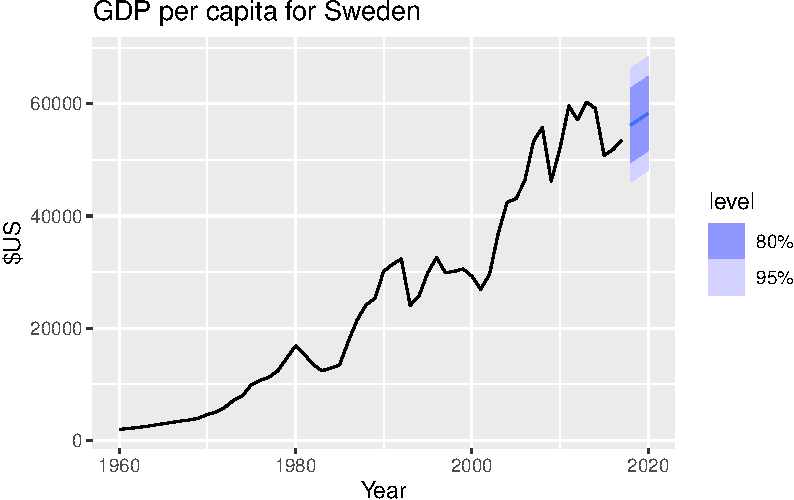
\includegraphics{chapter5_review_files/figure-pdf/unnamed-chunk-7-1.pdf}
\end{center}

Notice that the plot also contains 80\% and 95\% confidence levels (or
intervals) for your forecasts, as represented by the dark blue and light
blue ranges, respectively.

\section{Mean method}\label{mean-method}

The mean method of forecasting simply produces forecasts for future
periods that are equal to the mean of the time series considered.

\phantomsection\label{annotated-cell-8}%
\begin{Shaded}
\begin{Highlighting}[]
\NormalTok{recent\_prod }\OtherTok{\textless{}{-}} \FunctionTok{filter\_index}\NormalTok{(aus\_production, }\StringTok{"1970 Q1"} \SpecialCharTok{\textasciitilde{}} \StringTok{"2004 Q4"}\NormalTok{)}
\NormalTok{bricks }\OtherTok{\textless{}{-}}\NormalTok{ dplyr}\SpecialCharTok{::}\FunctionTok{select}\NormalTok{(recent\_prod, Bricks)}
\NormalTok{mean\_fit }\OtherTok{\textless{}{-}} \FunctionTok{model}\NormalTok{(bricks, }\FunctionTok{MEAN}\NormalTok{(Bricks)) }\hspace*{\fill}\NormalTok{\circled{1}}
\end{Highlighting}
\end{Shaded}

\begin{description}
\tightlist
\item[\circled{1}]
This is how you specify that you want to use the \texttt{MEAN()} method
for forecasting. As its argument you pass in the name of the column for
which you want to get the forecasts (\texttt{Bricks} in this case)
\end{description}

\begin{Shaded}
\begin{Highlighting}[]
\FunctionTok{tidy}\NormalTok{(mean\_fit)  }\CommentTok{\# extract output (1)}
\end{Highlighting}
\end{Shaded}

\begin{verbatim}
# A tibble: 1 x 6
  .model       term  estimate std.error statistic   p.value
  <chr>        <chr>    <dbl>     <dbl>     <dbl>     <dbl>
1 MEAN(Bricks) mean      451.      5.34      84.4 2.58e-121
\end{verbatim}

Using the \texttt{tidy()} function you can have a look at a brief report
of the mean\_fit model. You can see specifically that the estimate is
equal to the mean of the time series considered. Also, you get the
p-value which tells you about the significance of the model. Since the
p-value is very close to 0, this model is statistically significant and
we can use it to produce forecasts.

\begin{Shaded}
\begin{Highlighting}[]
\NormalTok{results\_list }\OtherTok{\textless{}{-}}\NormalTok{ mean\_fit}\SpecialCharTok{$}\StringTok{\textquotesingle{}MEAN(Bricks)\textquotesingle{}}\NormalTok{[[}\DecValTok{1}\NormalTok{]] }\CommentTok{\# extract output (2)}
\NormalTok{mean\_results }\OtherTok{\textless{}{-}}\NormalTok{ results\_list}\SpecialCharTok{$}\NormalTok{fit}

\NormalTok{mean\_fc }\OtherTok{\textless{}{-}} \FunctionTok{forecast}\NormalTok{(mean\_fit, }\AttributeTok{h =} \DecValTok{12}\NormalTok{)}
\NormalTok{bricks\_mean }\OtherTok{=} \FunctionTok{mutate}\NormalTok{(bricks,}\AttributeTok{hline=}\NormalTok{mean\_fc}\SpecialCharTok{$}\NormalTok{.mean[}\DecValTok{1}\NormalTok{]) }\CommentTok{\# add a dashed line}
\FunctionTok{autoplot}\NormalTok{(mean\_fc, bricks, }\AttributeTok{level =} \ConstantTok{NULL}\NormalTok{) }\SpecialCharTok{+}
  \FunctionTok{autolayer}\NormalTok{(bricks\_mean,hline,}\AttributeTok{linetype=}\StringTok{\textquotesingle{}dashed\textquotesingle{}}\NormalTok{,}\AttributeTok{color=}\StringTok{\textquotesingle{}blue\textquotesingle{}}\NormalTok{)}
\end{Highlighting}
\end{Shaded}

\begin{center}
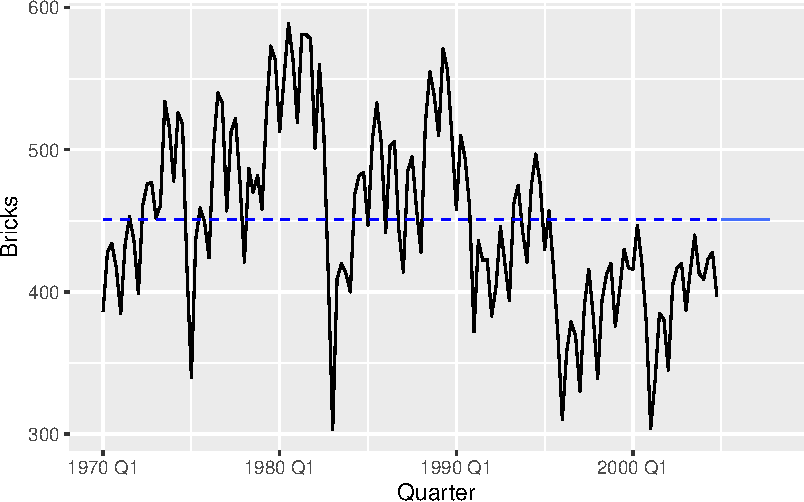
\includegraphics{chapter5_review_files/figure-pdf/unnamed-chunk-10-1.pdf}
\end{center}

The lines of code above produce the plot that shows that the forecasts
are indeed equal to the mean of the time series.

\section{Naive method}\label{naive-method}

This method produces forecasts that are just equal to the last observed
value in the time series.

\phantomsection\label{annotated-cell-11}%
\begin{Shaded}
\begin{Highlighting}[]
\NormalTok{naive\_fit }\OtherTok{\textless{}{-}} \FunctionTok{model}\NormalTok{(bricks,}\FunctionTok{NAIVE}\NormalTok{(Bricks)) }\hspace*{\fill}\NormalTok{\circled{1}}
\end{Highlighting}
\end{Shaded}

\begin{description}
\tightlist
\item[\circled{1}]
Specify the \texttt{NAIVE()} model and fit it to the data
\end{description}

\phantomsection\label{annotated-cell-12}%
\begin{Shaded}
\begin{Highlighting}[]
\NormalTok{naive\_fc }\OtherTok{\textless{}{-}} \FunctionTok{forecast}\NormalTok{(naive\_fit, }\AttributeTok{h =} \DecValTok{12}\NormalTok{) }\hspace*{\fill}\NormalTok{\circled{1}}
\end{Highlighting}
\end{Shaded}

\begin{description}
\tightlist
\item[\circled{1}]
Produce forecasts using the model specified
\end{description}

\begin{Shaded}
\begin{Highlighting}[]
\FunctionTok{autoplot}\NormalTok{(naive\_fc, bricks, }\AttributeTok{level =} \ConstantTok{NULL}\NormalTok{)}
\end{Highlighting}
\end{Shaded}

\begin{center}
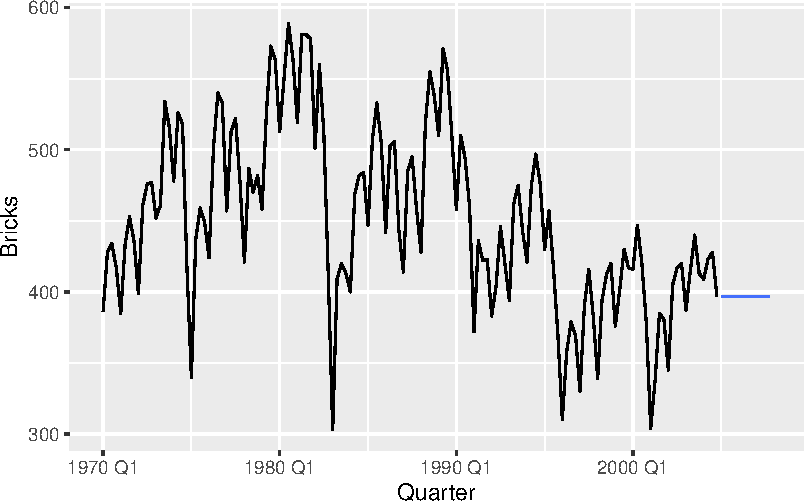
\includegraphics{chapter5_review_files/figure-pdf/unnamed-chunk-13-1.pdf}
\end{center}

The plot above just shows how the forecasts produced with this method
are equal to the last value observed in the series.

\section{Seasonal Naive}\label{seasonal-naive}

This method is similar to the Naive method but produces forecasts in the
future that are equal to the last seasonal trend observed in the data.

\phantomsection\label{annotated-cell-14}%
\begin{Shaded}
\begin{Highlighting}[]
\NormalTok{snaive\_fit }\OtherTok{\textless{}{-}} \FunctionTok{model}\NormalTok{(bricks,}\FunctionTok{SNAIVE}\NormalTok{(Bricks }\SpecialCharTok{\textasciitilde{}} \FunctionTok{lag}\NormalTok{(}\StringTok{"year"}\NormalTok{))) }\hspace*{\fill}\NormalTok{\circled{1}}
\end{Highlighting}
\end{Shaded}

\begin{description}
\tightlist
\item[\circled{1}]
specify \texttt{SNAIVE()} model indicating that the seasonal trend is
observed at a yearly interval
\end{description}

\begin{Shaded}
\begin{Highlighting}[]
\NormalTok{snaive\_fc }\OtherTok{\textless{}{-}} \FunctionTok{forecast}\NormalTok{(snaive\_fit, }\AttributeTok{h =} \DecValTok{12}\NormalTok{)}
\end{Highlighting}
\end{Shaded}

\phantomsection\label{annotated-cell-16}%
\begin{Shaded}
\begin{Highlighting}[]
\FunctionTok{autoplot}\NormalTok{(snaive\_fc, bricks, }\AttributeTok{level =} \ConstantTok{NULL}\NormalTok{) }\hspace*{\fill}\NormalTok{\circled{1}}
\end{Highlighting}
\end{Shaded}

\begin{description}
\tightlist
\item[\circled{1}]
Here the \texttt{level} argument is set to \texttt{NULL} so that the
plot does not contain forecast confidence intervals
\end{description}

\begin{center}
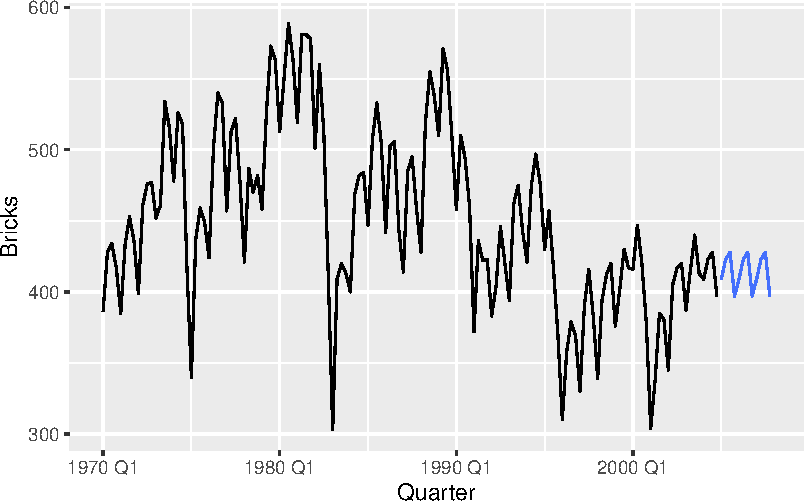
\includegraphics{chapter5_review_files/figure-pdf/unnamed-chunk-16-1.pdf}
\end{center}

\begin{Shaded}
\begin{Highlighting}[]
\NormalTok{bricks }\SpecialCharTok{\%\textgreater{}\%}
  \FunctionTok{filter\_index}\NormalTok{(}\StringTok{"Q1 2004"}\SpecialCharTok{\textasciitilde{}}\StringTok{"Q4 2004"}\NormalTok{) }\SpecialCharTok{\%\textgreater{}\%}
  \FunctionTok{autoplot}\NormalTok{(}\AttributeTok{.vars =}\NormalTok{ Bricks)}
\end{Highlighting}
\end{Shaded}

\begin{center}
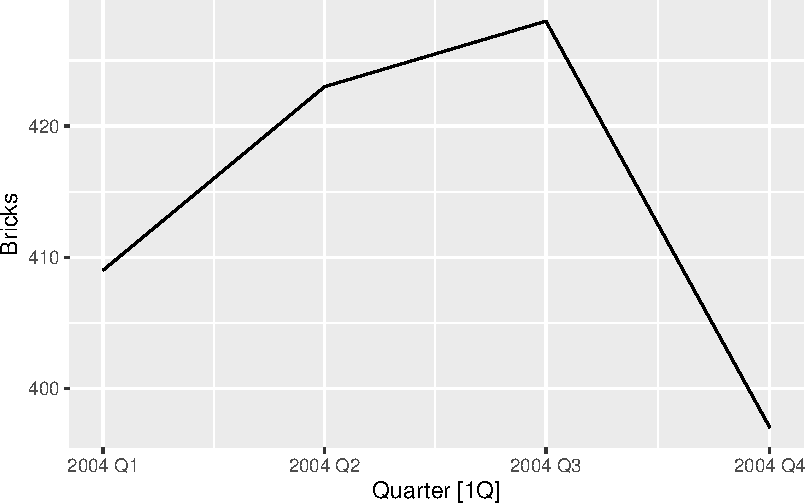
\includegraphics{chapter5_review_files/figure-pdf/unnamed-chunk-17-1.pdf}
\end{center}

Notice that the yearly trend looks something like the plot above, which
is exactly the shape that the future forecasts follow.

\section{Drift method}\label{drift-method}

This method interpolates between the first and last observation and the
line obtained is then ``stretched'' into future periods to produce
forecasts.

\begin{Shaded}
\begin{Highlighting}[]
\NormalTok{drift\_fit }\OtherTok{\textless{}{-}} \FunctionTok{model}\NormalTok{(bricks, }\FunctionTok{RW}\NormalTok{(Bricks }\SpecialCharTok{\textasciitilde{}} \FunctionTok{drift}\NormalTok{()))}
\NormalTok{drift\_fc }\OtherTok{\textless{}{-}} \FunctionTok{forecast}\NormalTok{(drift\_fit, }\AttributeTok{h =} \DecValTok{12}\NormalTok{)}
\FunctionTok{autoplot}\NormalTok{(drift\_fc, bricks, }\AttributeTok{level =} \ConstantTok{NULL}\NormalTok{)}
\end{Highlighting}
\end{Shaded}

\begin{center}
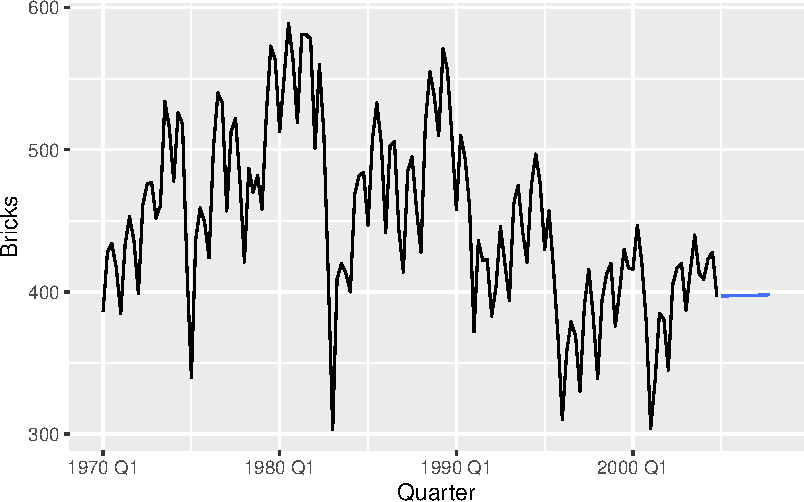
\includegraphics{chapter5_review_files/figure-pdf/unnamed-chunk-18-1.pdf}
\end{center}

To have a basic idea of how this works, we can convince ourselves that
the line used in the forecast is actually the line going from the first
to the last observation by looking at this plot.

\begin{Shaded}
\begin{Highlighting}[]
\NormalTok{T }\OtherTok{\textless{}{-}} \FunctionTok{length}\NormalTok{(bricks}\SpecialCharTok{$}\NormalTok{Bricks) }\CommentTok{\#getting length of Bricks column}
\NormalTok{b }\OtherTok{\textless{}{-}}\NormalTok{ (bricks}\SpecialCharTok{$}\NormalTok{Bricks[T] }\SpecialCharTok{{-}}\NormalTok{ bricks}\SpecialCharTok{$}\NormalTok{Bricks[}\DecValTok{1}\NormalTok{])}\SpecialCharTok{/}\NormalTok{(T }\SpecialCharTok{{-}} \DecValTok{1}\NormalTok{) }\CommentTok{\#equation of a line: slope (row140{-}row1)/(140{-}1)}
\NormalTok{a }\OtherTok{\textless{}{-}}\NormalTok{ bricks}\SpecialCharTok{$}\NormalTok{Bricks[}\DecValTok{1}\NormalTok{] }
\NormalTok{y }\OtherTok{\textless{}{-}}\NormalTok{ a }\SpecialCharTok{+}\NormalTok{ b }\SpecialCharTok{*} \FunctionTok{seq}\NormalTok{(}\DecValTok{1}\NormalTok{,T,}\AttributeTok{by=}\DecValTok{1}\NormalTok{)}

\NormalTok{DashDR }\OtherTok{\textless{}{-}} \FunctionTok{tibble}\NormalTok{(y,}\AttributeTok{Date=}\NormalTok{bricks}\SpecialCharTok{$}\NormalTok{Quarter)}
\NormalTok{DashDRts }\OtherTok{\textless{}{-}} \FunctionTok{as\_tsibble}\NormalTok{(DashDR,}\AttributeTok{index=}\NormalTok{Date)}

\FunctionTok{autoplot}\NormalTok{(drift\_fc, bricks, }\AttributeTok{level =} \ConstantTok{NULL}\NormalTok{)}\SpecialCharTok{+}
  \FunctionTok{autolayer}\NormalTok{(DashDRts,y,}\AttributeTok{color=}\StringTok{\textquotesingle{}blue\textquotesingle{}}\NormalTok{,}\AttributeTok{linetype=}\StringTok{\textquotesingle{}dashed\textquotesingle{}}\NormalTok{)}
\end{Highlighting}
\end{Shaded}

\begin{center}
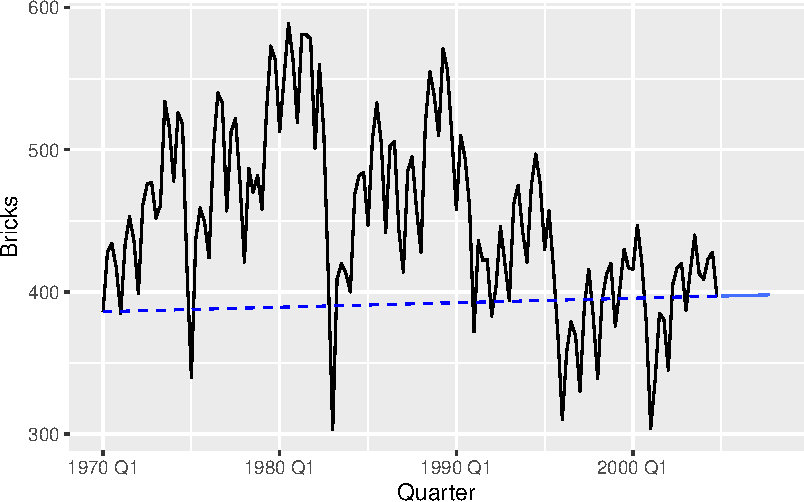
\includegraphics{chapter5_review_files/figure-pdf/unnamed-chunk-19-1.pdf}
\end{center}

\begin{tcolorbox}[enhanced jigsaw, toptitle=1mm, titlerule=0mm, leftrule=.75mm, opacityback=0, breakable, colback=white, bottomrule=.15mm, rightrule=.15mm, left=2mm, toprule=.15mm, bottomtitle=1mm, title=\textcolor{quarto-callout-tip-color}{\faLightbulb}\hspace{0.5em}{Tip \ref*{tip-slope}: Equation of a line}, arc=.35mm, colbacktitle=quarto-callout-tip-color!10!white, opacitybacktitle=0.6, coltitle=black, colframe=quarto-callout-tip-color-frame]

\quartocallouttip{tip-slope} 

Notice that T, b, a are used to compute the interpolated line and that
this follows from the equation of a line of the form \(y = mx + q\)
where \(m\) is the slope parameter (b in the code) and \(q\) is the
intercept (a in the code, which is just the first observation in the
time series).

\end{tcolorbox}

\section{Train / Test Split}\label{train-test-split}

To test how well our model performs we need to test in on data on which
it was not trained. This is often done to prevent the problem of
\emph{overfitting} which refers to the fact that when a parameters of a
model are estimated those perform well on the data that the model has
already seen but performs poorly on new data (which is actually what
should not happen). To mitigate this problem we divide our dataset into
a \emph{train} and a \emph{test} portion.

\phantomsection\label{annotated-cell-20}%
\begin{Shaded}
\begin{Highlighting}[]
\NormalTok{train }\OtherTok{\textless{}{-}} \FunctionTok{filter\_index}\NormalTok{(aus\_production, }\StringTok{"1992 Q1"} \SpecialCharTok{\textasciitilde{}} \StringTok{"2006 Q4"}\NormalTok{) }\hspace*{\fill}\NormalTok{\circled{1}}
\end{Highlighting}
\end{Shaded}

\begin{description}
\tightlist
\item[\circled{1}]
Our train dataset is made only of observations from 1992 to 2006.
\end{description}

\phantomsection\label{annotated-cell-21}%
\begin{Shaded}
\begin{Highlighting}[]
\NormalTok{beer\_fit }\OtherTok{\textless{}{-}} \FunctionTok{model}\NormalTok{(train, }\AttributeTok{Mean =} \FunctionTok{MEAN}\NormalTok{(Beer), }\AttributeTok{Naive =} \FunctionTok{NAIVE}\NormalTok{(Beer),}
\StringTok{\textquotesingle{}Seasonal naive\textquotesingle{}} \OtherTok{=} \FunctionTok{SNAIVE}\NormalTok{(Beer)) }\hspace*{\fill}\NormalTok{\circled{1}}
\NormalTok{beer\_fc }\OtherTok{\textless{}{-}} \FunctionTok{forecast}\NormalTok{(beer\_fit, }\AttributeTok{h =} \DecValTok{14}\NormalTok{) }\hspace*{\fill}\NormalTok{\circled{2}}
\end{Highlighting}
\end{Shaded}

\begin{description}
\tightlist
\item[\circled{1}]
fit three different models using the MEAN, NAIVE, and SNAIVE methods
\item[\circled{2}]
produce forecasts based on these three models
\end{description}

\begin{Shaded}
\begin{Highlighting}[]
\FunctionTok{autoplot}\NormalTok{(beer\_fc, train, }\AttributeTok{level =} \ConstantTok{NULL}\NormalTok{) }\SpecialCharTok{+}
  \FunctionTok{autolayer}\NormalTok{(}\FunctionTok{filter\_index}\NormalTok{(aus\_production, }\StringTok{"2007 Q1"} \SpecialCharTok{\textasciitilde{}}\NormalTok{ .), }\AttributeTok{.vars =}\NormalTok{ Beer,}
  \AttributeTok{colour =} \StringTok{"black"}\NormalTok{) }\SpecialCharTok{+} \FunctionTok{labs}\NormalTok{(}\AttributeTok{y =} \StringTok{"Megalitres"}\NormalTok{, }\AttributeTok{title =} \StringTok{"Forecasts}
\StringTok{            for quarterly beer production"}\NormalTok{) }\SpecialCharTok{+}
  \FunctionTok{guides}\NormalTok{(}\AttributeTok{colour =} \FunctionTok{guide\_legend}\NormalTok{(}\AttributeTok{title =} \StringTok{"Forecast"}\NormalTok{))}
\end{Highlighting}
\end{Shaded}

\begin{center}
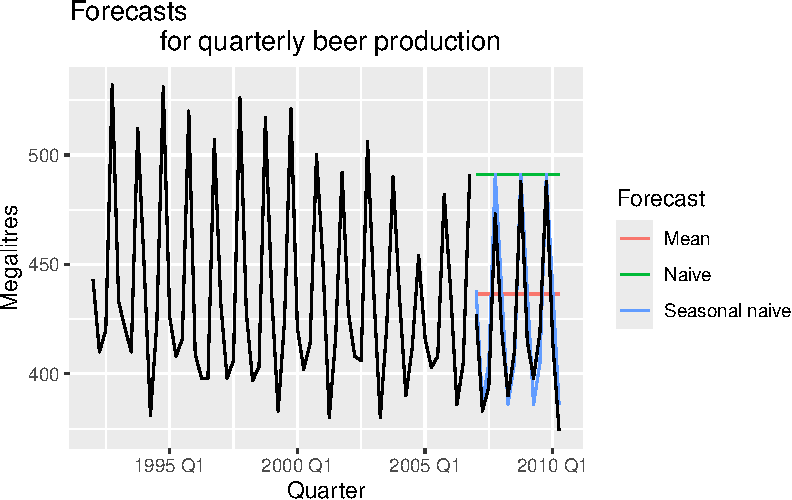
\includegraphics{chapter5_review_files/figure-pdf/unnamed-chunk-22-1.pdf}
\end{center}

Now we can plot how well the three different models perform and we can
see that the Seasonal Naive produces more accurate forecasts as it is
closer to the original series (black line). Notice, that by the way they
were constructed, the models did not see all the data in the series but
they were trained only on data up to 2006. Nonetheless, the Seasonal
Naive performs pretty well when it tries to make forecasts on data it
did not see. In a later section we will see how we can quantify how well
a model performs.

\subsection{More Examples}\label{more-examples}

\phantomsection\label{annotated-cell-23}%
\begin{Shaded}
\begin{Highlighting}[]
\NormalTok{recent\_GOOG }\OtherTok{\textless{}{-}} \FunctionTok{filter}\NormalTok{(gafa\_stock, Symbol }\SpecialCharTok{==} \StringTok{"GOOG"}\NormalTok{,}
                      \FunctionTok{year}\NormalTok{(Date) }\SpecialCharTok{\textgreater{}=} \DecValTok{2015}\NormalTok{)}

\NormalTok{goog }\OtherTok{\textless{}{-}} \FunctionTok{mutate}\NormalTok{(recent\_GOOG, }\AttributeTok{day =} \FunctionTok{row\_number}\NormalTok{()) }\hspace*{\fill}\NormalTok{\circled{1}}

\NormalTok{google\_stock }\OtherTok{\textless{}{-}} \FunctionTok{update\_tsibble}\NormalTok{(goog, }\AttributeTok{index =}\NormalTok{ day, }\AttributeTok{regular =} \ConstantTok{TRUE}\NormalTok{)}

\NormalTok{google\_2015 }\OtherTok{\textless{}{-}} \FunctionTok{filter}\NormalTok{(google\_stock, }\FunctionTok{year}\NormalTok{(Date) }\SpecialCharTok{==} \DecValTok{2015}\NormalTok{) }\CommentTok{\# Filter the year of interest}

\NormalTok{google\_fit }\OtherTok{\textless{}{-}} \FunctionTok{model}\NormalTok{(google\_2015, }\CommentTok{\# Fit the models}
\AttributeTok{Mean =} \FunctionTok{MEAN}\NormalTok{(Close), }\AttributeTok{Naive =} \FunctionTok{NAIVE}\NormalTok{(Close),}
\AttributeTok{Drift =} \FunctionTok{NAIVE}\NormalTok{(Close }\SpecialCharTok{\textasciitilde{}} \FunctionTok{drift}\NormalTok{()))}
\end{Highlighting}
\end{Shaded}

\begin{description}
\tightlist
\item[\circled{1}]
the \texttt{row\_number()} function adds a sequence of numbers
representing the row number of each observation (basically a sequence,
starts from 1 and ends with the last observation)
\end{description}

By now you should be able to see what's going on in these lines of code.
We are filtering, mutating and updating the original tsibble to take as
index the day column we just created before. The last three lines is
where we fit models to data.

\phantomsection\label{annotated-cell-24}%
\begin{Shaded}
\begin{Highlighting}[]
\NormalTok{google\_jan\_2016 }\OtherTok{\textless{}{-}} \FunctionTok{filter}\NormalTok{(google\_stock,}
        \FunctionTok{yearmonth}\NormalTok{(Date) }\SpecialCharTok{==} \FunctionTok{yearmonth}\NormalTok{(}\StringTok{"2016 Jan"}\NormalTok{)) }\hspace*{\fill}\NormalTok{\circled{1}}

\NormalTok{(google\_fc }\OtherTok{\textless{}{-}} \FunctionTok{forecast}\NormalTok{(google\_fit, }\AttributeTok{new\_data =}\NormalTok{ google\_jan\_2016)) }\hspace*{\fill}\NormalTok{\circled{2}}
\end{Highlighting}
\end{Shaded}

\begin{description}
\tightlist
\item[\circled{1}]
Produce forecasts for the trading days in January 2016
\item[\circled{2}]
the \texttt{new\_data} argument is used to specify for which datapoints
the forecasts should be produced. In this example, we will be producing
forecasts only for the trading days in Jan 2016
\end{description}

\begin{verbatim}
# A fable: 57 x 11 [1]
# Key:     Symbol, .model [3]
   Symbol .model   day
   <chr>  <chr>  <int>
 1 GOOG   Mean     253
 2 GOOG   Mean     254
 3 GOOG   Mean     255
 4 GOOG   Mean     256
 5 GOOG   Mean     257
 6 GOOG   Mean     258
 7 GOOG   Mean     259
 8 GOOG   Mean     260
 9 GOOG   Mean     261
10 GOOG   Mean     262
# i 47 more rows
# i 8 more variables: Close <dist>, .mean <dbl>, Date <date>, Open <dbl>,
#   High <dbl>, Low <dbl>, Adj_Close <dbl>, Volume <dbl>
\end{verbatim}

\phantomsection\label{annotated-cell-25}%
\begin{Shaded}
\begin{Highlighting}[]
\FunctionTok{autoplot}\NormalTok{(google\_fc, google\_2015, }\AttributeTok{level =} \ConstantTok{NULL}\NormalTok{) }\SpecialCharTok{+}
  \FunctionTok{autolayer}\NormalTok{(google\_jan\_2016, Close, }\AttributeTok{colour =} \StringTok{"black"}\NormalTok{) }\SpecialCharTok{+} \hspace*{\fill}\NormalTok{\circled{1}}
  \FunctionTok{labs}\NormalTok{(}\AttributeTok{y =} \StringTok{"$US"}\NormalTok{, }\AttributeTok{title =} \StringTok{"Google daily closing stock prices"}\NormalTok{,}
       \AttributeTok{subtitle =} \StringTok{"(Jan 2015 {-} Jan 2016)"}\NormalTok{) }\SpecialCharTok{+}
  \FunctionTok{guides}\NormalTok{(}\AttributeTok{colour =} \FunctionTok{guide\_legend}\NormalTok{(}\AttributeTok{title =} \StringTok{"Forecast"}\NormalTok{))}
\end{Highlighting}
\end{Shaded}

\begin{description}
\tightlist
\item[\circled{1}]
Remember that \texttt{autolayer()} just adds another layer to the plot
produced with \texttt{autoplot()} instead of starting a new plot from a
white, empty canvas.
\end{description}

\begin{center}
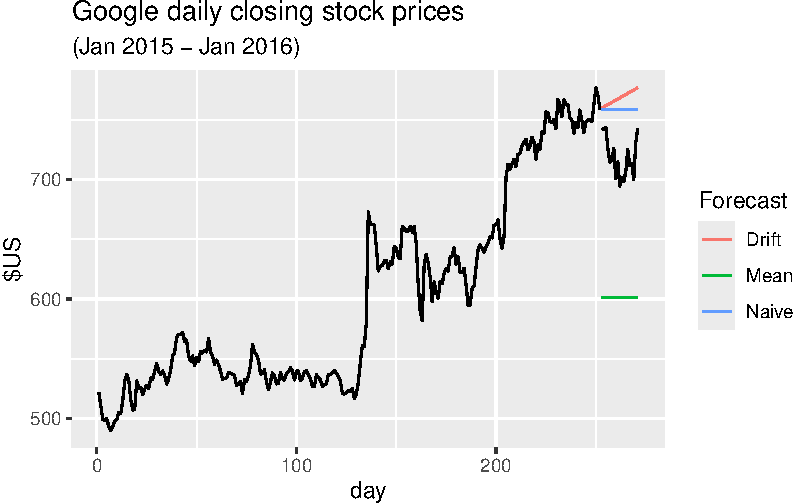
\includegraphics{chapter5_review_files/figure-pdf/unnamed-chunk-25-1.pdf}
\end{center}

The plot just shows what each model predicts for the Jan 2016 period.

\section{Residuals}\label{residuals}

Residuals are the errors that our model makes when being tested.
Basically, they represent the difference between the true observed value
and what the model predicted that value to be. We now start with an
example to understand how residuals fit in our discussion.

\phantomsection\label{annotated-cell-26}%
\begin{Shaded}
\begin{Highlighting}[]
\NormalTok{beer\_fit1 }\OtherTok{\textless{}{-}} \FunctionTok{model}\NormalTok{(train, }\FunctionTok{SNAIVE}\NormalTok{(Beer))}
\NormalTok{(mean\_fitted }\OtherTok{\textless{}{-}} \FunctionTok{augment}\NormalTok{(beer\_fit1)) }\hspace*{\fill}\NormalTok{\circled{1}}
\end{Highlighting}
\end{Shaded}

\begin{description}
\tightlist
\item[\circled{1}]
fitted values for a single method, along with residuals and innovation
residuals
\end{description}

\begin{verbatim}
# A tsibble: 60 x 6 [1Q]
# Key:       .model [1]
   .model       Quarter  Beer .fitted .resid .innov
   <chr>          <qtr> <dbl>   <dbl>  <dbl>  <dbl>
 1 SNAIVE(Beer) 1992 Q1   443      NA     NA     NA
 2 SNAIVE(Beer) 1992 Q2   410      NA     NA     NA
 3 SNAIVE(Beer) 1992 Q3   420      NA     NA     NA
 4 SNAIVE(Beer) 1992 Q4   532      NA     NA     NA
 5 SNAIVE(Beer) 1993 Q1   433     443    -10    -10
 6 SNAIVE(Beer) 1993 Q2   421     410     11     11
 7 SNAIVE(Beer) 1993 Q3   410     420    -10    -10
 8 SNAIVE(Beer) 1993 Q4   512     532    -20    -20
 9 SNAIVE(Beer) 1994 Q1   449     433     16     16
10 SNAIVE(Beer) 1994 Q2   381     421    -40    -40
# i 50 more rows
\end{verbatim}

We saw how by using \texttt{augment()} on a model we previously fit to
our data we can get some more information about how it performs. For
instance, we can see that the .resid and .innovation column contain the
residuals and the innovation residuals for each estimate provided by the
model. The difference between residuals and innovation residuals is just
that innovation residuals are more interpretable when dealing with data
that has gone through transformations. However, since that was not the
case with our example, we see that the residuals match perfectly with
the innovation ones.

\begin{Shaded}
\begin{Highlighting}[]
\FunctionTok{ggplot}\NormalTok{(mean\_fitted, }\FunctionTok{aes}\NormalTok{(}\AttributeTok{x =}\NormalTok{ Quarter)) }\SpecialCharTok{+}
  \FunctionTok{geom\_line}\NormalTok{(}\FunctionTok{aes}\NormalTok{(}\AttributeTok{y =}\NormalTok{ Beer),}\AttributeTok{color=}\StringTok{\textquotesingle{}black\textquotesingle{}}\NormalTok{) }\SpecialCharTok{+}
  \FunctionTok{geom\_line}\NormalTok{(}\FunctionTok{aes}\NormalTok{(}\AttributeTok{y =}\NormalTok{ .fitted),}\AttributeTok{color=}\StringTok{\textquotesingle{}red\textquotesingle{}}\NormalTok{) }
\end{Highlighting}
\end{Shaded}

\begin{center}
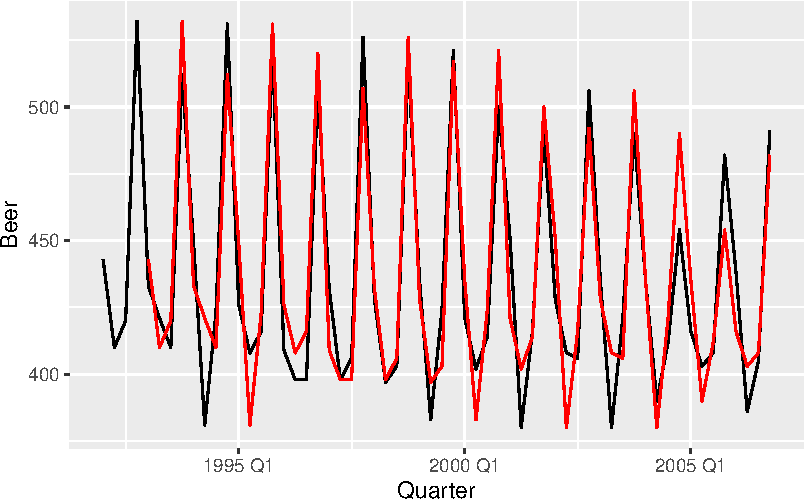
\includegraphics{chapter5_review_files/figure-pdf/unnamed-chunk-27-1.pdf}
\end{center}

\begin{Shaded}
\begin{Highlighting}[]
\FunctionTok{autoplot}\NormalTok{(mean\_fitted,}\AttributeTok{.vars =}\NormalTok{ Beer) }\SpecialCharTok{+} \CommentTok{\# alternative command}
  \FunctionTok{autolayer}\NormalTok{(mean\_fitted,.fitted,}\AttributeTok{color=}\StringTok{\textquotesingle{}red\textquotesingle{}}\NormalTok{)}
\end{Highlighting}
\end{Shaded}

\begin{center}
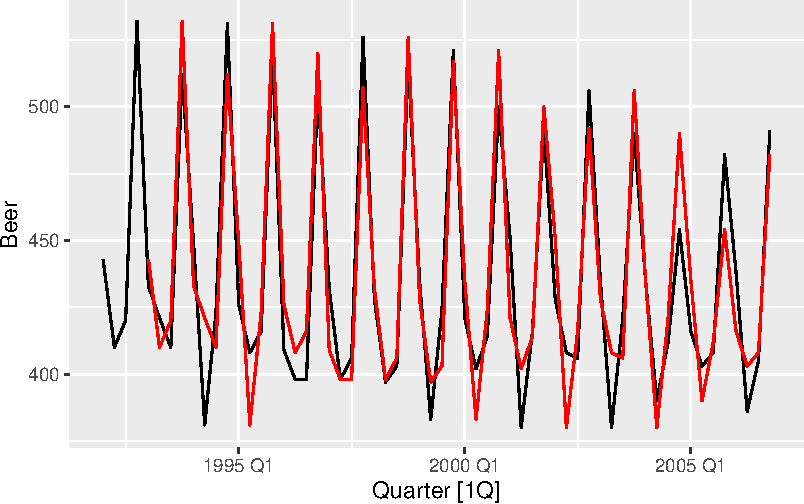
\includegraphics{chapter5_review_files/figure-pdf/unnamed-chunk-27-2.pdf}
\end{center}

In the plot we see that the predictions produced are very close to the
actual series, meaning that the model performs well on the data.

\begin{Shaded}
\begin{Highlighting}[]
\FunctionTok{gg\_tsresiduals}\NormalTok{(beer\_fit1)}
\end{Highlighting}
\end{Shaded}

\begin{center}
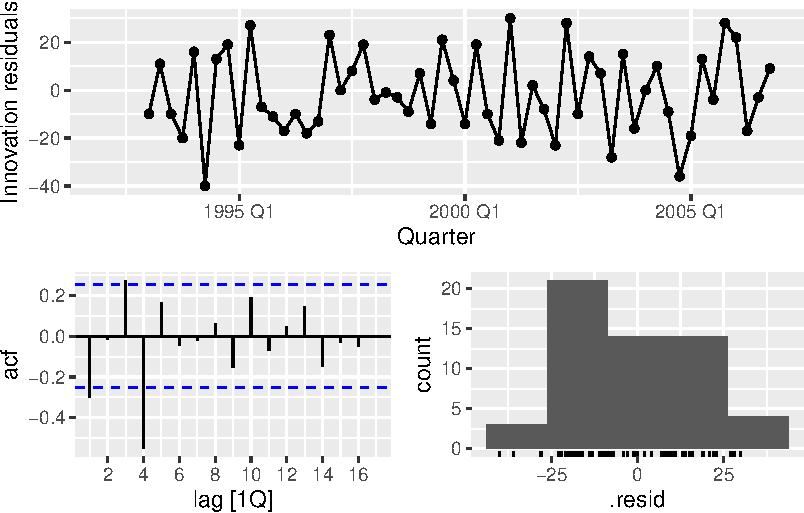
\includegraphics{chapter5_review_files/figure-pdf/unnamed-chunk-28-1.pdf}
\end{center}

The \texttt{gg\_tsresiduals()} is a very useful function that allows you
to check different assumptions that are imposed on residuals through
plots. The usual assumption that are imposed on residuals is that they
exhibit:

\begin{enumerate}
\def\labelenumi{\arabic{enumi}.}
\tightlist
\item
  \href{https://en.wikipedia.org/wiki/Homoscedasticity_and_heteroscedasticity}{homoskedasticity}
  (or exhibit no heteroskedasticity), meaning that there should be no
  visible pattern in how residuals are distributed over time. This is
  visible from the plot at the top.
\item
  no significant
  \href{https://en.wikipedia.org/wiki/Autocorrelation}{autocorrelation},
  this follows from the first assumption as autocorrelation would imply
  a pattern in the time series that should be exploited but that our
  model does not capture. You can check this assumption from the ACF
  plot on the bottom left.
\item
  residuals are normally distributed, you can check this from the
  histogram at the bottom right.
\end{enumerate}

\subsection{Assumptions on Residuals
(continued)}\label{assumptions-on-residuals-continued}

We continue the discussion here more in-depth.

\begin{Shaded}
\begin{Highlighting}[]
\NormalTok{aug }\OtherTok{\textless{}{-}} \FunctionTok{augment}\NormalTok{(}\FunctionTok{model}\NormalTok{(google\_2015, }\FunctionTok{NAIVE}\NormalTok{(Close)))}
\FunctionTok{autoplot}\NormalTok{(aug, .innov) }\SpecialCharTok{+}
  \FunctionTok{labs}\NormalTok{(}\AttributeTok{y =} \StringTok{"$US"}\NormalTok{, }\AttributeTok{title =} \StringTok{"Residuals from the Naive method"}\NormalTok{)}
\end{Highlighting}
\end{Shaded}

\begin{center}
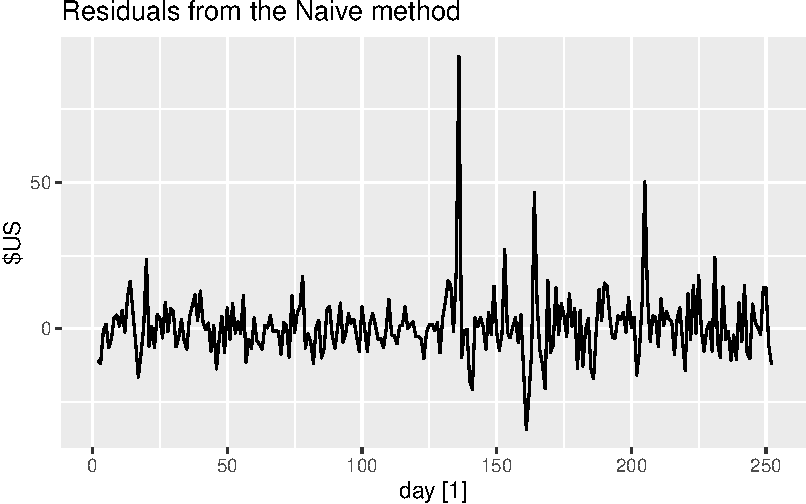
\includegraphics{chapter5_review_files/figure-pdf/unnamed-chunk-29-1.pdf}
\end{center}

In the plot is a graphical representation of the residuals throughout
the entire model we estimated using the NAIVE method.

We can also check that the distribution of the residuals closely mirrors
a normal distribution with the following lines of code

\phantomsection\label{annotated-cell-31}%
\begin{Shaded}
\begin{Highlighting}[]
\NormalTok{p0 }\OtherTok{\textless{}{-}} \FunctionTok{ggplot}\NormalTok{(aug, }\FunctionTok{aes}\NormalTok{(}\AttributeTok{x =}\NormalTok{ .innov)) }\SpecialCharTok{+}
  \FunctionTok{geom\_histogram}\NormalTok{(}\FunctionTok{aes}\NormalTok{(}\AttributeTok{y=}\FunctionTok{after\_stat}\NormalTok{(density)), }\AttributeTok{bins =} \DecValTok{20}\NormalTok{, }\hspace*{\fill}\NormalTok{\circled{1}}
  \AttributeTok{color=}\StringTok{"black"}\NormalTok{, }\AttributeTok{fill=}\StringTok{"white"}\NormalTok{)}

\NormalTok{p0 }\SpecialCharTok{+} \FunctionTok{stat\_function}\NormalTok{(}\AttributeTok{fun =}\NormalTok{ dnorm, }\AttributeTok{colour =} \StringTok{"red"}\NormalTok{, }\hspace*{\fill}\NormalTok{\circled{2}}
  \AttributeTok{args =} \FunctionTok{list}\NormalTok{(}\AttributeTok{mean =} \FunctionTok{mean}\NormalTok{(aug}\SpecialCharTok{$}\NormalTok{.innov,}\AttributeTok{na.rm=}\ConstantTok{TRUE}\NormalTok{),}
  \AttributeTok{sd =} \FunctionTok{sd}\NormalTok{(aug}\SpecialCharTok{$}\NormalTok{.innov,}\AttributeTok{na.rm=}\ConstantTok{TRUE}\NormalTok{)))}
\end{Highlighting}
\end{Shaded}

\begin{description}
\tightlist
\item[\circled{1}]
The \texttt{after\_stat()} function used as a y \texttt{aesthetic}
inside the \texttt{geom\_histogram()} layer of the ggplot, is used to
specify that we want the \texttt{density} to be plotted on the y axis as
opposed to the default behavior of the function which is to plot the
\texttt{count}.
\item[\circled{2}]
The \texttt{stat\_function()} is used to add a layer which plots a
probability distribution specified by the argument \texttt{fun}. In this
case, we are plotting the density of the normal distribution
(\texttt{dnorm()}) in red. Since it is another layer, it is superimposed
to the histogram. Since each normal distribution is uniquely identified
by a \texttt{mean} and a \texttt{standard\ deviation}, we need to pass
these values inside the \texttt{dnorm()} function using the
\texttt{args} argument as a \texttt{list}.
\end{description}

\begin{center}
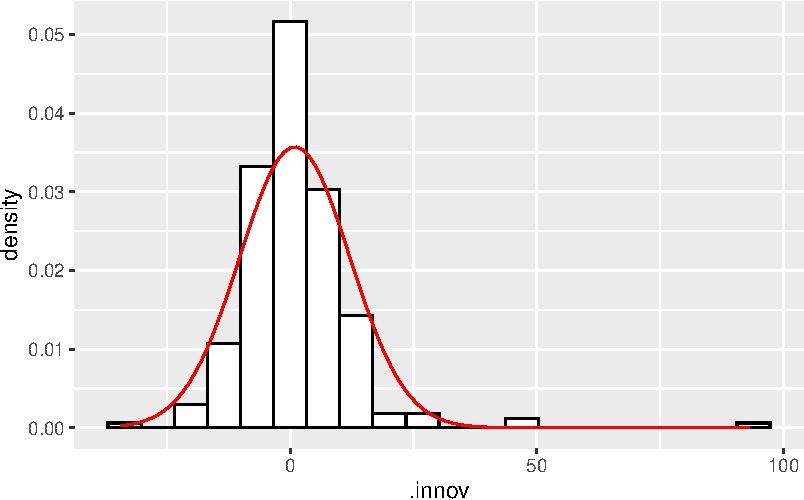
\includegraphics{chapter5_review_files/figure-pdf/unnamed-chunk-30-1.pdf}
\end{center}

\begin{Shaded}
\begin{Highlighting}[]
\FunctionTok{autoplot}\NormalTok{(}\FunctionTok{ACF}\NormalTok{(aug, .innov)) }\SpecialCharTok{+}
  \FunctionTok{labs}\NormalTok{(}\AttributeTok{title =} \StringTok{"Residuals from the Naive method"}\NormalTok{)}
\end{Highlighting}
\end{Shaded}

\begin{center}
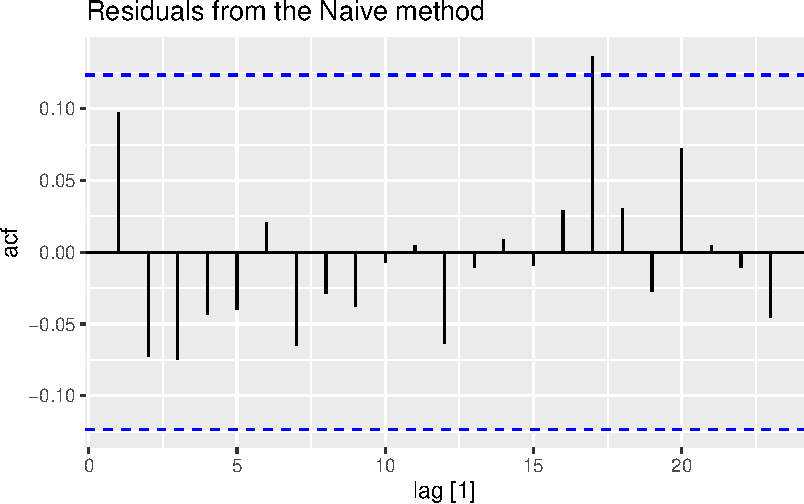
\includegraphics{chapter5_review_files/figure-pdf/unnamed-chunk-31-1.pdf}
\end{center}

By computing the ACF we can also plot it and check for the presence of
significant autocorrelation of residuals at different time lags.

\subsection{Portmanteau Tests}\label{portmanteau-tests}

These kinds of test are used when we want to assess the level of
autocorrelation in a time series across a number \(k\) of lags, where
\(k \in \mathbb{N}\) (i.e., notation for saying that \(k\) is a
\href{https://www.cuemath.com/numbers/natural-numbers/}{natural
number}). There are two main tests that your book discusses.

\subsubsection{Box-Pierce Test}\label{box-pierce-test}

\begin{Shaded}
\begin{Highlighting}[]
\FunctionTok{features}\NormalTok{(aug, .innov, box\_pierce, }\AttributeTok{lag =} \DecValTok{10}\NormalTok{)}
\end{Highlighting}
\end{Shaded}

\begin{verbatim}
# A tibble: 1 x 4
  Symbol .model       bp_stat bp_pvalue
  <chr>  <chr>          <dbl>     <dbl>
1 GOOG   NAIVE(Close)    7.74     0.654
\end{verbatim}

With this we compute the Box-Pierce statistic on the data and obtain its
related p-value. Generally a p-value greater than 0.1 will be a good way
of assessing that the residuals are randomly distributed and that there
is no significant pattern arising from their actual distribution.

\subsubsection{Ljung-Box Test}\label{ljung-box-test}

\begin{Shaded}
\begin{Highlighting}[]
\FunctionTok{features}\NormalTok{(aug, .innov, ljung\_box, }\AttributeTok{lag =} \DecValTok{10}\NormalTok{)}
\end{Highlighting}
\end{Shaded}

\begin{verbatim}
# A tibble: 1 x 4
  Symbol .model       lb_stat lb_pvalue
  <chr>  <chr>          <dbl>     <dbl>
1 GOOG   NAIVE(Close)    7.91     0.637
\end{verbatim}

Another approach is using the Ljung-Box test. It has been shown that the
two tests yield comparable results, however, this test has been shown to
be more precise overall so it is recommended that you use this one from
now on. Remember that to use the \texttt{features()} function you need
to specify the augmented model fit (\texttt{aug} in the example), select
the \texttt{.innov} column containing the innovation residuals, and then
specify that you want to compute the \texttt{ljung\_box} statistic with
a \texttt{lag} of 10 (due to the data being non-seasonal in this case).

\begin{tcolorbox}[enhanced jigsaw, toptitle=1mm, titlerule=0mm, leftrule=.75mm, opacityback=0, breakable, colback=white, bottomrule=.15mm, rightrule=.15mm, left=2mm, toprule=.15mm, bottomtitle=1mm, title=\textcolor{quarto-callout-important-color}{\faExclamation}\hspace{0.5em}{Important}, arc=.35mm, colbacktitle=quarto-callout-important-color!10!white, opacitybacktitle=0.6, coltitle=black, colframe=quarto-callout-important-color-frame]

The book suggests using ℓ=10 (i.e., \texttt{lag\ =\ 10}) for
non-seasonal data and ℓ=2m for seasonal data, where m is the period of
seasonality. However, the test is not good when ℓ is large, so if these
values are larger than T/5, then use ℓ=T/5. T in this case refers to the
total number of observations that you are using to carry out the test
(i.e., number of rows in your dataset).

\end{tcolorbox}

\paragraph{More examples}\label{more-examples-1}

We can now use this method to check if the residuals produced by other
models present patterns or are auto-correlated.

\phantomsection\label{annotated-cell-35}%
\begin{Shaded}
\begin{Highlighting}[]
\NormalTok{fit }\OtherTok{\textless{}{-}} \FunctionTok{model}\NormalTok{(google\_2015, }\FunctionTok{RW}\NormalTok{(Close }\SpecialCharTok{\textasciitilde{}} \FunctionTok{drift}\NormalTok{()))}
\FunctionTok{tidy}\NormalTok{(fit) }\hspace*{\fill}\NormalTok{\circled{1}}
\end{Highlighting}
\end{Shaded}

\begin{description}
\tightlist
\item[\circled{1}]
remember that the estimate obtained using the drift method is
\(\frac{(y_{T}-y_{1})}{(T-1)}\) = (759-522)/251 = 0.9439931. We saw this
also in Tip~\ref{tip-slope}
\end{description}

\begin{verbatim}
# A tibble: 1 x 7
  Symbol .model              term  estimate std.error statistic p.value
  <chr>  <chr>               <chr>    <dbl>     <dbl>     <dbl>   <dbl>
1 GOOG   RW(Close ~ drift()) b        0.944     0.705      1.34   0.182
\end{verbatim}

\begin{Shaded}
\begin{Highlighting}[]
\FunctionTok{features}\NormalTok{(}\FunctionTok{augment}\NormalTok{(fit), .innov, ljung\_box, }\AttributeTok{lag=}\DecValTok{10}\NormalTok{)}
\end{Highlighting}
\end{Shaded}

\begin{verbatim}
# A tibble: 1 x 4
  Symbol .model              lb_stat lb_pvalue
  <chr>  <chr>                 <dbl>     <dbl>
1 GOOG   RW(Close ~ drift())    7.91     0.637
\end{verbatim}

then we compute the Ljung Box statistic and see that the p-value is
\textgreater{} .1 and therefore we can assume that residuals are
randomly distributed (no pattern)

\begin{Shaded}
\begin{Highlighting}[]
\FunctionTok{hilo}\NormalTok{(}\FunctionTok{forecast}\NormalTok{(}\FunctionTok{model}\NormalTok{(google\_2015, }\FunctionTok{NAIVE}\NormalTok{(Close)), }\AttributeTok{h =} \DecValTok{10}\NormalTok{))}
\end{Highlighting}
\end{Shaded}

\begin{verbatim}
# A tsibble: 10 x 7 [1]
# Key:       Symbol, .model [1]
   Symbol .model         day
   <chr>  <chr>        <dbl>
 1 GOOG   NAIVE(Close)   253
 2 GOOG   NAIVE(Close)   254
 3 GOOG   NAIVE(Close)   255
 4 GOOG   NAIVE(Close)   256
 5 GOOG   NAIVE(Close)   257
 6 GOOG   NAIVE(Close)   258
 7 GOOG   NAIVE(Close)   259
 8 GOOG   NAIVE(Close)   260
 9 GOOG   NAIVE(Close)   261
10 GOOG   NAIVE(Close)   262
# i 4 more variables: Close <dist>, .mean <dbl>, `80%` <hilo>, `95%` <hilo>
\end{verbatim}

Finally we use the \texttt{hilo()} function to extract confidence
(prediction) intervals for each prediction obtained from a NAIVE model.

\subsection{Bootstrapped residuals}\label{bootstrapped-residuals}

We can use our model to generate more observations. These observations
would be generated based on what has been observed in previous periods,
but they would still vary. In this case, we are building a simulation to
test our model on multiple different future possibilities. The method
that is used to obtain new random observations starting from a sample is
called \textbf{bootstrap}.

To generate these bootstrapped residuals we can use the
\texttt{generate()} function in R. Alternatively, we could also just set
the \texttt{bootstrap} argument in the \texttt{forecast()} to
\texttt{TRUE} and specify how many \texttt{times} we want to run the
bootstrap simulation.

\phantomsection\label{annotated-cell-38}%
\begin{Shaded}
\begin{Highlighting}[]
\NormalTok{(fore }\OtherTok{\textless{}{-}} \FunctionTok{forecast}\NormalTok{(}\FunctionTok{model}\NormalTok{(google\_2015, }\FunctionTok{NAIVE}\NormalTok{(Close)), }\AttributeTok{h =} \DecValTok{10}\NormalTok{,}
        \AttributeTok{bootstrap =} \ConstantTok{TRUE}\NormalTok{, }\AttributeTok{times =} \DecValTok{1000}\NormalTok{)) }\hspace*{\fill}\NormalTok{\circled{1}}
\end{Highlighting}
\end{Shaded}

\begin{description}
\tightlist
\item[\circled{1}]
This specifies that the bootstrapping process will perform 1000
simulations. Each simulation generates a possible future path for the
time series. These simulations are then aggregated to produce the final
forecast distribution.
\end{description}

\begin{verbatim}
# A fable: 10 x 5 [1]
# Key:     Symbol, .model [1]
   Symbol .model         day        Close .mean
   <chr>  <chr>        <dbl>       <dist> <dbl>
 1 GOOG   NAIVE(Close)   253 sample[1000]  759.
 2 GOOG   NAIVE(Close)   254 sample[1000]  759.
 3 GOOG   NAIVE(Close)   255 sample[1000]  759.
 4 GOOG   NAIVE(Close)   256 sample[1000]  758.
 5 GOOG   NAIVE(Close)   257 sample[1000]  758.
 6 GOOG   NAIVE(Close)   258 sample[1000]  759.
 7 GOOG   NAIVE(Close)   259 sample[1000]  759.
 8 GOOG   NAIVE(Close)   260 sample[1000]  759.
 9 GOOG   NAIVE(Close)   261 sample[1000]  759.
10 GOOG   NAIVE(Close)   262 sample[1000]  759.
\end{verbatim}

Finally we take a look at the final forecast distribution along with the
prediction intervals

\begin{Shaded}
\begin{Highlighting}[]
\FunctionTok{hilo}\NormalTok{(fore)}
\end{Highlighting}
\end{Shaded}

\begin{verbatim}
# A tsibble: 10 x 7 [1]
# Key:       Symbol, .model [1]
   Symbol .model         day        Close .mean                  `80%`
   <chr>  <chr>        <dbl>       <dist> <dbl>                 <hilo>
 1 GOOG   NAIVE(Close)   253 sample[1000]  759. [747.3290, 769.8360]80
 2 GOOG   NAIVE(Close)   254 sample[1000]  759. [741.6050, 774.2036]80
 3 GOOG   NAIVE(Close)   255 sample[1000]  759. [738.2767, 779.7247]80
 4 GOOG   NAIVE(Close)   256 sample[1000]  758. [733.8743, 782.1182]80
 5 GOOG   NAIVE(Close)   257 sample[1000]  758. [731.4141, 786.1595]80
 6 GOOG   NAIVE(Close)   258 sample[1000]  759. [728.6593, 790.6161]80
 7 GOOG   NAIVE(Close)   259 sample[1000]  759. [726.1230, 793.6760]80
 8 GOOG   NAIVE(Close)   260 sample[1000]  759. [723.3868, 795.5324]80
 9 GOOG   NAIVE(Close)   261 sample[1000]  759. [721.3646, 798.3353]80
10 GOOG   NAIVE(Close)   262 sample[1000]  759. [718.7703, 800.8452]80
# i 1 more variable: `95%` <hilo>
\end{verbatim}

\section{Final lines of code}\label{final-lines-of-code}

\subsection{More examples on model fitting and diagnosis of
residuals}\label{more-examples-on-model-fitting-and-diagnosis-of-residuals}

\phantomsection\label{annotated-cell-40}%
\begin{Shaded}
\begin{Highlighting}[]
\NormalTok{us\_retail\_employment }\OtherTok{\textless{}{-}} \FunctionTok{filter}\NormalTok{(us\_employment, }\FunctionTok{year}\NormalTok{(Month) }\SpecialCharTok{\textgreater{}=} \DecValTok{1990}\NormalTok{,}
\NormalTok{                        Title }\SpecialCharTok{==} \StringTok{"Retail Trade"}\NormalTok{) }\hspace*{\fill}\NormalTok{\circled{1}}

\NormalTok{US\_model\_0 }\OtherTok{\textless{}{-}} \FunctionTok{model}\NormalTok{(us\_retail\_employment,}
              \FunctionTok{STL}\NormalTok{(Employed }\SpecialCharTok{\textasciitilde{}} \FunctionTok{trend}\NormalTok{(}\AttributeTok{window =} \DecValTok{7}\NormalTok{), }\AttributeTok{robust =} \ConstantTok{TRUE}\NormalTok{)) }\hspace*{\fill}\NormalTok{\circled{2}}
\end{Highlighting}
\end{Shaded}

\begin{description}
\tightlist
\item[\circled{1}]
filter the dataset
\item[\circled{2}]
specify the model formula using an STL-based decomposition using only
the trend component
\end{description}

\phantomsection\label{annotated-cell-41}%
\begin{Shaded}
\begin{Highlighting}[]
\NormalTok{US\_model\_1 }\OtherTok{\textless{}{-}} \FunctionTok{select}\NormalTok{(}\FunctionTok{components}\NormalTok{(US\_model\_0), }\SpecialCharTok{{-}}\NormalTok{.model) }\hspace*{\fill}\NormalTok{\circled{1}}

\NormalTok{(US\_fore }\OtherTok{\textless{}{-}} \FunctionTok{forecast}\NormalTok{(}\FunctionTok{model}\NormalTok{(US\_model\_1, }\FunctionTok{NAIVE}\NormalTok{(season\_adjust)))) }\hspace*{\fill}\NormalTok{\circled{2}}
\end{Highlighting}
\end{Shaded}

\begin{description}
\tightlist
\item[\circled{1}]
get rid of the \texttt{.model} column
\item[\circled{2}]
produce forecasts using the NAIVE method on the seasonally adjusted
series
\end{description}

\begin{verbatim}
# A fable: 24 x 5 [1M]
# Key:     Series_ID, .model [1]
   Series_ID     .model                  Month
   <chr>         <chr>                   <mth>
 1 CEU4200000001 NAIVE(season_adjust) 2019 Oct
 2 CEU4200000001 NAIVE(season_adjust) 2019 Nov
 3 CEU4200000001 NAIVE(season_adjust) 2019 Dec
 4 CEU4200000001 NAIVE(season_adjust) 2020 Jan
 5 CEU4200000001 NAIVE(season_adjust) 2020 Feb
 6 CEU4200000001 NAIVE(season_adjust) 2020 Mar
 7 CEU4200000001 NAIVE(season_adjust) 2020 Apr
 8 CEU4200000001 NAIVE(season_adjust) 2020 May
 9 CEU4200000001 NAIVE(season_adjust) 2020 Jun
10 CEU4200000001 NAIVE(season_adjust) 2020 Jul
# i 14 more rows
# i 2 more variables: season_adjust <dist>, .mean <dbl>
\end{verbatim}

Finally, we plot the results from our model which is based on seasonally
adjusted data.

\begin{Shaded}
\begin{Highlighting}[]
\FunctionTok{autoplot}\NormalTok{(US\_fore, US\_model\_1) }\SpecialCharTok{+}
  \FunctionTok{labs}\NormalTok{(}\AttributeTok{y =} \StringTok{"Number of people"}\NormalTok{, }\AttributeTok{title =} \StringTok{"US retail employment"}\NormalTok{)}
\end{Highlighting}
\end{Shaded}

\begin{center}
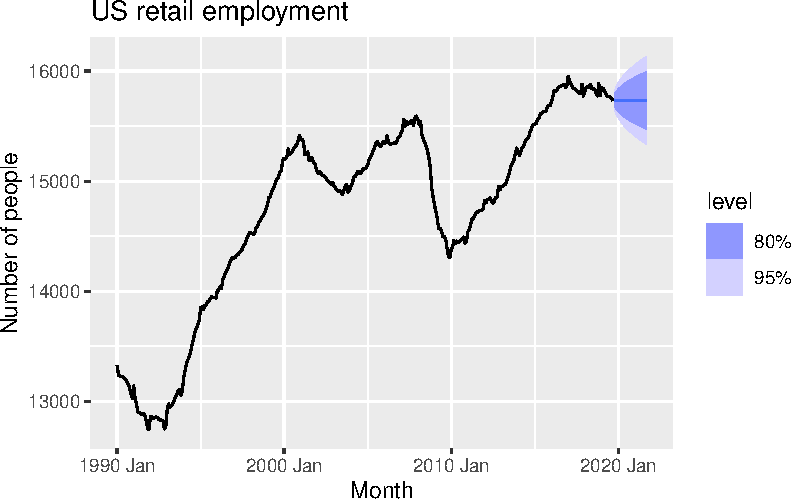
\includegraphics{chapter5_review_files/figure-pdf/unnamed-chunk-41-1.pdf}
\end{center}

Another similar example follows below.

\begin{Shaded}
\begin{Highlighting}[]
\NormalTok{fit\_dcmp }\OtherTok{\textless{}{-}} \FunctionTok{model}\NormalTok{(us\_retail\_employment,}
    \AttributeTok{stlf =} \FunctionTok{decomposition\_model}\NormalTok{(}\FunctionTok{STL}\NormalTok{(Employed }\SpecialCharTok{\textasciitilde{}} \FunctionTok{trend}\NormalTok{(}\AttributeTok{window =} \DecValTok{7}\NormalTok{),}
          \AttributeTok{robust =} \ConstantTok{TRUE}\NormalTok{), }\FunctionTok{NAIVE}\NormalTok{(season\_adjust)))}
\end{Highlighting}
\end{Shaded}

We start from the decomposing the model using an STL decomposition as
before and then we fit a NAIVE model to the seasonally adjusted time
series. We then plot the results.

\begin{Shaded}
\begin{Highlighting}[]
\FunctionTok{autoplot}\NormalTok{(}\FunctionTok{forecast}\NormalTok{(fit\_dcmp), us\_retail\_employment) }\SpecialCharTok{+}
  \FunctionTok{labs}\NormalTok{(}\AttributeTok{y =} \StringTok{"Number of people"}\NormalTok{, }\AttributeTok{title =} \StringTok{"Monthly US retail employment"}\NormalTok{)}
\end{Highlighting}
\end{Shaded}

\begin{center}
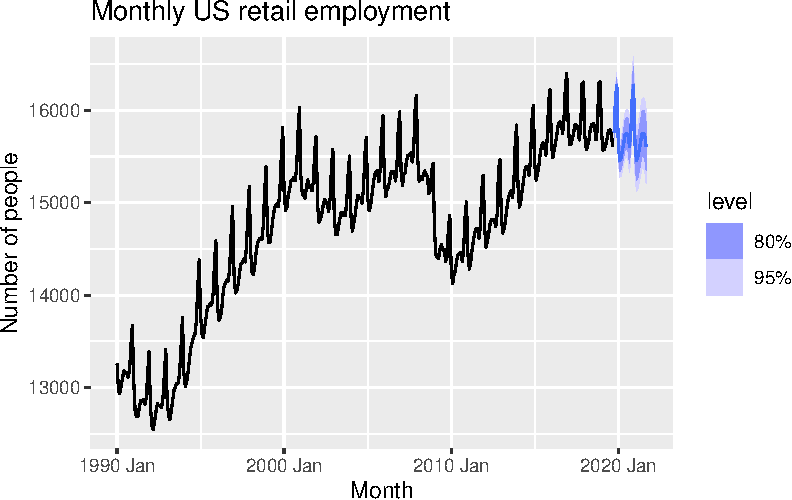
\includegraphics{chapter5_review_files/figure-pdf/unnamed-chunk-43-1.pdf}
\end{center}

We can also plot the residuals of the model by using:

\begin{Shaded}
\begin{Highlighting}[]
\FunctionTok{gg\_tsresiduals}\NormalTok{(fit\_dcmp)}
\end{Highlighting}
\end{Shaded}

\begin{center}
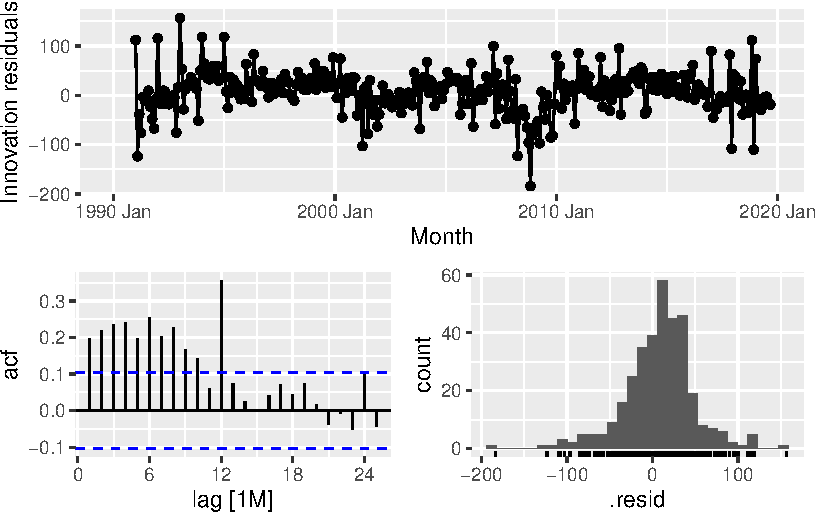
\includegraphics{chapter5_review_files/figure-pdf/unnamed-chunk-44-1.pdf}
\end{center}

From here we notice some patterns in how those are distributed and the
autocorrelation at different time lags. We now want to compute the mean
of the innovation residuals.

\begin{Shaded}
\begin{Highlighting}[]
\FunctionTok{features}\NormalTok{(}\FunctionTok{augment}\NormalTok{(fit\_dcmp), .innov, }\FunctionTok{list}\NormalTok{(}\AttributeTok{avg =} \SpecialCharTok{\textasciitilde{}} \FunctionTok{mean}\NormalTok{(.,}\AttributeTok{na.rm=}\ConstantTok{TRUE}\NormalTok{)))}
\end{Highlighting}
\end{Shaded}

\begin{verbatim}
# A tibble: 1 x 3
  Series_ID     .model   avg
  <chr>         <chr>  <dbl>
1 CEU4200000001 stlf    7.84
\end{verbatim}

A simpler way to get the mean of the residuals \textbf{when you only
estimate one model} is shown below.

\begin{Shaded}
\begin{Highlighting}[]
\FunctionTok{mean}\NormalTok{(}\FunctionTok{augment}\NormalTok{(fit\_dcmp)}\SpecialCharTok{$}\NormalTok{.innov, }\AttributeTok{na.rm=}\ConstantTok{TRUE}\NormalTok{)}
\end{Highlighting}
\end{Shaded}

\begin{verbatim}
[1] 7.836419
\end{verbatim}

\subsection{Subsetting}\label{subsetting}

Subsetting refers to extracting only some rows in a dataset. Subsetting
is usually a synonym of filtering the data and this is also shown in
code. Here is an example:

\phantomsection\label{annotated-cell-48}%
\begin{Shaded}
\begin{Highlighting}[]
\FunctionTok{filter}\NormalTok{(aus\_production, }\FunctionTok{year}\NormalTok{(Quarter) }\SpecialCharTok{\textgreater{}=} \DecValTok{1995}\NormalTok{) }\hspace*{\fill}\NormalTok{\circled{1}}
\end{Highlighting}
\end{Shaded}

\begin{description}
\tightlist
\item[\circled{1}]
only get the rows where the year of the observation is greater than or
equal to 1995
\end{description}

\begin{verbatim}
# A tsibble: 62 x 7 [1Q]
   Quarter  Beer Tobacco Bricks Cement Electricity   Gas
     <qtr> <dbl>   <dbl>  <dbl>  <dbl>       <dbl> <dbl>
 1 1995 Q1   426    4714    430   1626       41768   131
 2 1995 Q2   408    3939    457   1703       43686   167
 3 1995 Q3   416    6137    417   1733       46022   181
 4 1995 Q4   520    4739    370   1545       42800   145
 5 1996 Q1   409    4275    310   1526       43661   133
 6 1996 Q2   398    5239    358   1593       44707   162
 7 1996 Q3   398    6293    379   1706       46326   184
 8 1996 Q4   507    5575    369   1699       43346   146
 9 1997 Q1   432    4802    330   1511       43938   135
10 1997 Q2   398    5523    390   1785       45828   171
# i 52 more rows
\end{verbatim}

In case you do not have a specific filtering condition to use, you can
use slice to get a subset of your data.

\phantomsection\label{annotated-cell-49}%
\begin{Shaded}
\begin{Highlighting}[]
\FunctionTok{slice}\NormalTok{(aus\_production, }\FunctionTok{n}\NormalTok{()}\SpecialCharTok{{-}}\DecValTok{19}\SpecialCharTok{:}\DecValTok{0}\NormalTok{) }\hspace*{\fill}\NormalTok{\circled{1}}
\end{Highlighting}
\end{Shaded}

\begin{description}
\tightlist
\item[\circled{1}]
last 20 observations obtained using the \texttt{n()} function which
returns the total number of rows (n) in the aus\_production dataset.
Then the slice only selects the rows from n-19 to the end.
\end{description}

\begin{verbatim}
# A tsibble: 20 x 7 [1Q]
   Quarter  Beer Tobacco Bricks Cement Electricity   Gas
     <qtr> <dbl>   <dbl>  <dbl>  <dbl>       <dbl> <dbl>
 1 2005 Q3   408      NA     NA   2340       56043   221
 2 2005 Q4   482      NA     NA   2265       54992   180
 3 2006 Q1   438      NA     NA   2027       57112   171
 4 2006 Q2   386      NA     NA   2278       57157   224
 5 2006 Q3   405      NA     NA   2427       58400   233
 6 2006 Q4   491      NA     NA   2451       56249   192
 7 2007 Q1   427      NA     NA   2140       56244   187
 8 2007 Q2   383      NA     NA   2362       55036   234
 9 2007 Q3   394      NA     NA   2536       59806   245
10 2007 Q4   473      NA     NA   2562       56411   205
11 2008 Q1   420      NA     NA   2183       59118   194
12 2008 Q2   390      NA     NA   2558       56660   229
13 2008 Q3   410      NA     NA   2612       64067   249
14 2008 Q4   488      NA     NA   2373       59045   203
15 2009 Q1   415      NA     NA   1963       58368   196
16 2009 Q2   398      NA     NA   2160       57471   238
17 2009 Q3   419      NA     NA   2325       58394   252
18 2009 Q4   488      NA     NA   2273       57336   210
19 2010 Q1   414      NA     NA   1904       58309   205
20 2010 Q2   374      NA     NA   2401       58041   236
\end{verbatim}

\begin{Shaded}
\begin{Highlighting}[]
\FunctionTok{slice}\NormalTok{(}\FunctionTok{group\_by}\NormalTok{(aus\_retail, State, Industry), }\DecValTok{1}\SpecialCharTok{:}\DecValTok{12}\NormalTok{) }\CommentTok{\# working with groups}
\end{Highlighting}
\end{Shaded}

\begin{verbatim}
# A tsibble: 1,824 x 5 [1M]
# Key:       State, Industry [152]
# Groups:    State, Industry [152]
   State                        Industry           `Series ID`    Month Turnover
   <chr>                        <chr>              <chr>          <mth>    <dbl>
 1 Australian Capital Territory Cafes, restaurant~ A3349849A   1982 Apr      4.4
 2 Australian Capital Territory Cafes, restaurant~ A3349849A   1982 May      3.4
 3 Australian Capital Territory Cafes, restaurant~ A3349849A   1982 Jun      3.6
 4 Australian Capital Territory Cafes, restaurant~ A3349849A   1982 Jul      4  
 5 Australian Capital Territory Cafes, restaurant~ A3349849A   1982 Aug      3.6
 6 Australian Capital Territory Cafes, restaurant~ A3349849A   1982 Sep      4.2
 7 Australian Capital Territory Cafes, restaurant~ A3349849A   1982 Oct      4.8
 8 Australian Capital Territory Cafes, restaurant~ A3349849A   1982 Nov      5.4
 9 Australian Capital Territory Cafes, restaurant~ A3349849A   1982 Dec      6.9
10 Australian Capital Territory Cafes, restaurant~ A3349849A   1983 Jan      3.8
# i 1,814 more rows
\end{verbatim}

\subsection{Forecast errors}\label{forecast-errors}

\phantomsection\label{annotated-cell-51}%
\begin{Shaded}
\begin{Highlighting}[]
\NormalTok{recent\_production }\OtherTok{\textless{}{-}} \FunctionTok{filter}\NormalTok{(aus\_production, }\FunctionTok{year}\NormalTok{(Quarter) }\SpecialCharTok{\textgreater{}=} \DecValTok{1992}\NormalTok{) }\hspace*{\fill}\NormalTok{\circled{1}}

\NormalTok{beer\_train }\OtherTok{\textless{}{-}} \FunctionTok{filter}\NormalTok{(recent\_production, }\FunctionTok{year}\NormalTok{(Quarter) }\SpecialCharTok{\textless{}=} \DecValTok{2007}\NormalTok{) }\hspace*{\fill}\NormalTok{\circled{2}}
\end{Highlighting}
\end{Shaded}

\begin{description}
\tightlist
\item[\circled{1}]
get rows where year is after 1992 (included)
\item[\circled{2}]
train / test split
\end{description}

\begin{Shaded}
\begin{Highlighting}[]
\NormalTok{beer\_fit }\OtherTok{\textless{}{-}} \FunctionTok{model}\NormalTok{(beer\_train, }\AttributeTok{Mean =} \FunctionTok{MEAN}\NormalTok{(Beer),}
    \AttributeTok{Naive =} \FunctionTok{NAIVE}\NormalTok{(Beer),}
    \StringTok{\textquotesingle{}Seasonal naive\textquotesingle{}} \OtherTok{=} \FunctionTok{SNAIVE}\NormalTok{(Beer),}
    \AttributeTok{Drift =} \FunctionTok{RW}\NormalTok{(Beer }\SpecialCharTok{\textasciitilde{}} \FunctionTok{drift}\NormalTok{()))}
\end{Highlighting}
\end{Shaded}

Fit three models to our training dataset. Finally, produce forecasts
using our model.

\begin{Shaded}
\begin{Highlighting}[]
\NormalTok{(beer\_fc }\OtherTok{\textless{}{-}} \FunctionTok{forecast}\NormalTok{(beer\_fit, }\AttributeTok{h =} \DecValTok{10}\NormalTok{))}
\end{Highlighting}
\end{Shaded}

\begin{verbatim}
# A fable: 40 x 4 [1Q]
# Key:     .model [4]
   .model Quarter
   <chr>    <qtr>
 1 Mean   2008 Q1
 2 Mean   2008 Q2
 3 Mean   2008 Q3
 4 Mean   2008 Q4
 5 Mean   2009 Q1
 6 Mean   2009 Q2
 7 Mean   2009 Q3
 8 Mean   2009 Q4
 9 Mean   2010 Q1
10 Mean   2010 Q2
# i 30 more rows
# i 2 more variables: Beer <dist>, .mean <dbl>
\end{verbatim}

And plot the forecasts without plotting the prediction intervals (i.e.,
\texttt{level\ =\ NULL}).

\begin{Shaded}
\begin{Highlighting}[]
\FunctionTok{autoplot}\NormalTok{(beer\_fc, recent\_production, }\AttributeTok{level =} \ConstantTok{NULL}\NormalTok{) }\SpecialCharTok{+}
  \FunctionTok{labs}\NormalTok{(}\AttributeTok{y =} \StringTok{"Megalitres"}\NormalTok{, }\AttributeTok{title =} \StringTok{"Forecasts for quarterly beer production"}\NormalTok{) }\SpecialCharTok{+}
  \FunctionTok{guides}\NormalTok{(}\AttributeTok{colour =} \FunctionTok{guide\_legend}\NormalTok{(}\AttributeTok{title =} \StringTok{"Forecast"}\NormalTok{))}
\end{Highlighting}
\end{Shaded}

\begin{center}
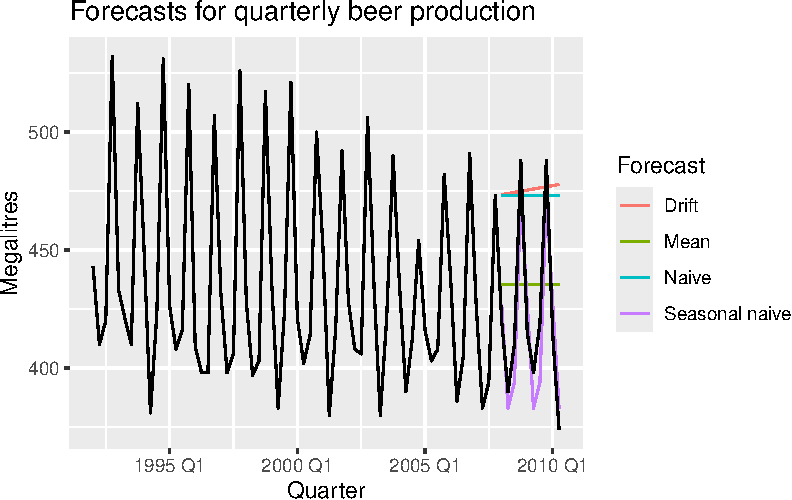
\includegraphics{chapter5_review_files/figure-pdf/unnamed-chunk-53-1.pdf}
\end{center}

Finally, we evaluate the performance of our model by producing an
accuracy table.

\begin{Shaded}
\begin{Highlighting}[]
\NormalTok{accTable }\OtherTok{\textless{}{-}} \FunctionTok{accuracy}\NormalTok{(beer\_fc, recent\_production)}
\FunctionTok{select}\NormalTok{(accTable,.model,RMSE,MAE,MAPE)}
\end{Highlighting}
\end{Shaded}

\begin{verbatim}
# A tibble: 4 x 4
  .model          RMSE   MAE  MAPE
  <chr>          <dbl> <dbl> <dbl>
1 Drift           64.9  58.9 14.6 
2 Mean            38.4  34.8  8.28
3 Naive           62.7  57.4 14.2 
4 Seasonal naive  14.3  13.4  3.17
\end{verbatim}

This allows us to get the main accuracy measures for the different
models fit to the data. From the table we see that the Seasonal naive
model scores the lowest on the error metrics, and therefore is the best
model among those proposed.




\end{document}
